% ----------------------------------------------------------------- %
%                     LATEX Thesis Template	              		    %
%                                                                   %
%		         		Version 1.6.1                       	    %
% ----------------------------------------------------------------- %

% ----------------------------------------------------------------- %
% Prepared by ITU Informatics Institute	                            %
%                                                                   %
% Informatics Institute, ITU Ayazaga Campus                         %
% Maslak-34469, İstanbul, Turkey									%
% http://www.be.itu.edu.tr											%
% ----------------------------------------------------------------- %

% ----------------------------------------------------------------- %
% Updated by	  :													%
% E. Baris Ondes  : ondes@itu.edu.tr 	OR ondesalt@pm.me			% 
% Tamer Sener	  : senerta@itu.edu.tr  OR senertam@pm.me			%
% Berkan Kacmaz	  : kacmazb@itu.edu.tr  OR kacmazberkan0@gmail.com	%
% S. Baris Ozturk : ozturksb@itu.edu.tr OR salihbaris@gmail.com		%
% ----------------------------------------------------------------- %

% ----------------------------------------------------------------- %
% Please visit the following page for the current version:			%
% https://github.com/ondes/Template-Latex-ITU-Thesis   				%
% ----------------------------------------------------------------- %

% ----------------------------------------------------------------- %
% documentclass arguments:             							    %
% [onluarkali,tekyonlu],[turkce,ingilizce],						    %
% [lisans,yukseklisans,doktora], [bez,karton],					    %
% [bilisim,fenbilimleri,sosyalbilimler,avrasya,enerji]			   	%
% Sample use: \documentclass[onluarkali,ingilizce,yukseklisans,    	%
% karton,fenbilimleri]{itutez}					  				   	%
% Other sample use: \documentclass[tekyonlu,ingilizce,	           	%
% yukseklisans,bez,bilisim]{itutez}			           			   	%
% onluarkali: twoside                     			  			   	%
% tekyonlu: oneside						 						   	%
% turkce: turkish						 						   	%
% ingilizce: english											   	%
% yukseklisans: masters											   	%
% doktora: phd							  						   	%
% bez: hardcover version					  					    %
% karton: paperback version					  					    %
% bilisim: informatics						  					    %
% fenbilimleri: science and technology							    %
% sosyalbilimler: social sciences				 				    %
% avrasya: eurasia						 						    %
% enerji: energy						   						    %
% elektrikelektronik: electrical and electronics				    %
% ----------------------------------------------------------------- %

\documentclass[onluarkali,ingilizce,yukseklisans,bez,fenbilimleri]{thesis_itu}

% ----------------------------------------------------------------- %
% Pay attention to letter case. The structure is case sensitive     %
% {Name}{SURNAME} means first letter of name is capital and that    %
% all letters of surname are capital.                               %
% ----------------------------------------------------------------- %

% ----------------------------------------------------------------- %
% No titles, only Name and SURNAME must be written.      	        %
% ----------------------------------------------------------------- %

\yazar{Name}{SURNAME}
\ogrencino{101010101}

% ----------------------------------------------------------------- %
% If you do not use the structure, do not delete it. Just delete    %
% the argument. \unvan{} means title.                               %
% ----------------------------------------------------------------- %

\unvan{(Any Profession)}
 
% ----------------------------------------------------------------- %
% For below, the first argument for Turkish, the second is for      %
% English.       						   						    %
% ----------------------------------------------------------------- %

% ----------------------------------------------------------------- %
% Only the first letters of words must be capital.		     	    %
% ----------------------------------------------------------------- %

\anabilimdali{Elektrik Mühendisliği Anabilim Dalı}{Department of Electrical Engineering}
\programi{Elektrik Mühendisliği Programı}{Electrical Engineering Programme}

% ----------------------------------------------------------------- %
% For paperback version, the submission date to the faculty. For    %
% hardcover (indigo/black) version, date of defense.		   	    %
% ----------------------------------------------------------------- %

\tarih{TEZİN SAVUNULDUĞU AY YIL}{MONTH YEAR OF DEFENSE}
\tarihKucuk{Tezin savunulduğu ay yıl}{Month year of defense}

% ----------------------------------------------------------------- %
% Thesis advisor, title, thesis submission date, defense date       %
% ----------------------------------------------------------------- %

\tezyoneticisi{Prof. Dr. Name SURNAME}{Istanbul Technical University}   

\baslik{TEZ BAŞLIĞI BURAYA GELİR}
{GEREKLİ İSE İKİNCİ SATIR}
{GEREKLİ İSE ÜÇÜNCÜ SATIR, ÜÇ SATIRA SIĞDIRINIZ}

\title{THESIS TITLE HERE}
{SECOND LINE IF NECESSARY}
{THIRD LINE IF NECESSARY, FIT TITLE IN THREE LINES}

% ----------------------------------------------------------------- %
% The date of submission of the paperback to the department.	    %
% ----------------------------------------------------------------- %

\tezvermetarih{1 Mayıs 2020}{1 May 2020} 

\tezsavunmatarih{1 Haziran 2020}{1 June 2020}

% ----------------------------------------------------------------- %
% coadvisor and jury information. If you do not use all items,     	%
% leave the corresponding arguments blank such as                  	%
% \esdanismani{}{} 					           						%
% ----------------------------------------------------------------- %

\esdanismani{Prof. Dr. Name SURNAME}{Istanbul Technical University}   

\juriBir{Prof. Dr. Name SURNAME}{Middle East Technical University}  

\juriIki{Prof. Dr. Name SURNAME}{Boğaziçi University}  

\juriUc{Prof. Dr. Name SURNAME}{Bilkent University}  

\juriDort{Prof. Dr. Name SURNAME}{Sabancı University}  

\juriBes{Prof. Dr. Name SURNAME}{Koç University}

% ----------------------------------------------------------------- %
% Packages and definitions to be used are given in the following    %
% ----------------------------------------------------------------- %

%
\usepackage{color}
\usepackage{times}
\usepackage{amssymb,amsmath,mathptmx,amsbsy,bm}
\usepackage{caption}            %%
%\usepackage{floatflt}
%\usepackage[dvipdfm]{graphicx}
\usepackage{graphics}
\usepackage{wrapfig}
\usepackage{epsfig}
\usepackage{enumerate}
\usepackage{rotating}
\usepackage{multirow}
\usepackage{subfigure}
\usepackage{colortbl}
\usepackage{pstricks}
\usepackage{pst-plot}
\usepackage{cite}%
\usepackage{latexsym}           % 
%\usepackage{subeqn}
\usepackage{rotating}
%\usepackage{hyperref}
%\usepackage{url}
\usepackage{fixltx2e} % Bu paketi sembollerde text ler için subscript yazmakta yardımcı olması için ekliyoruz.
\usepackage[open,openlevel=1]{bookmark} % It is used to have bookmarks in the PDF file created


% \usepackage{textcomp}
% \usepackage{array}
% \usepackage{lscape}
%\usepackage{listings} % Required for insertion of code
% \usepackage{xcolor}
%\usepackage[colorlinks=true,linkcolor=blue,urlcolor=black,bookmarksopen=true]{hyperref}

%Bold Equation Number, Unbold Reference
%\makeatletter
%\def\tagform@#1{\maketag@@@{\bfseries(\ignorespaces#1\unskip\@@italiccorr)}}
%\renewcommand{\eqref}[1]{\textup{{\normalfont(\ref{#1}}\normalfont)}}
%\makeatother

%\renewcommand{\theequation}{{\bf\arabic{chapter}.\arabic{equation}}}

\def\be{\begin{equation}} %
\def\ee{\end{equation}}%
\def\beq{\begin{eqnarray}}%
\def\eeq{\end{eqnarray}}%
\def\bse{\begin{subequations}}%
\def\ese{\end{subequations}}%
\def\nonu{\nonumber}%
\def\psibar{\overline{\psi}} %
\def\Delslash{\partial\!\!\!\!\!/}%
\def\Gslash{G\!\!\!\!\!/}%
\def\Lmbdslash{\lambda\!\!\!\!\!/}%
\def\Jslash{J\!\!\!\!\!/}%
\def\pslash{p\!\!\!\!/}%
\def\qslash{q\!\!\!\!/}%
\def\kslash{k\!\!\!\!/}%
\def\[{\left[}
\def\]{\right]}
\def\({\left(}
\def\){\right)}

\def\Lag{{\cal L}}    % 
\def\D{{\cal D}}      % 
\def\H{{\cal H}}      % 
\def\Z{{\cal Z}}      % 
\def\S{{\textbf{S}}}  % 
\def\d{{\rm d}}%
\def\dt{{\rm{dt}}}%
\def\Tr{{\rm{Tr}}}%
\def\gm{\gamma^{\mu}}
\def\ga{\gamma^{\alpha}}
\def\gb{\gamma^{\beta}}
\def\gn{\gamma^{\nu}}
\def\gs{\gamma^{\sigma}}
\def\gl{\gamma^{\lambda}}
\def\gr{\gamma^{\rho}}
\def\gd{\gamma^{\delta}}


                                        

% ----------------------------------------------------------------- %
% For dedication page. Leave the argument blank if not used.	    %
% ----------------------------------------------------------------- %

\ithaf{To my family,}

% ----------------------------------------------------------------- %
% Form the below files						   					    %
% ----------------------------------------------------------------- %

\kisaltmalistesi{\begin{tabular}{@{}p{2cm}l}
{\bf{AIC}} & {\bf:} Akaike Information Criteria\\
{\bf ANN} & {\bf:} Artificial Neural Network\\
{\bf App} & {\bf:} Appendix\\
{\bf BP} & {\bf:} Backpropagation\\
{\bf CGI} & {\bf:} Common Gateway Interface\\
{\bf ESS} & {\bf:} Error sum-of-squares\\
{\bf GARCH} & {\bf:} Generalized Autoregressive Conditional Heteroskedasticity\\
{\bf GIS} & {\bf:} Geographic Information Systems\\
{\bf HCA} & {\bf:} Hierarchical Cluster Analysis\\
{\bf Mbps} & {\bf:} Megabits per second\\
{\bf St} & {\bf:} Station\\
{\bf SWAT} & {\bf:} Soil and Water Assessment Tool\\
{\bf UMN} & {\bf:} University of Minnesota\\
\end{tabular}

}
\sembollistesi{\begin{tabular}{@{}p{2cm}l}
{\bf{C}} & {\bf:} Capacitance\\
{\bf H} & {\bf:} The amount of heat\\
{\bf M\textsubscript{x},} {\bf M\textsubscript{y}} & {\bf:} Torque Components\\
{\bf N\textsubscript{x},} {\bf N\textsubscript{y},} {\bf N\textsubscript{z}} & {\bf:} Normal Power Components\\
{\bf q} & {\bf:} Phase load\\
{\bf t} & {\bf:} Time\\
{\bf u, v} & {\bf:} Displacement Vector Components\\
{\bf w} & {\bf:} Angular velocity\\
{\bf XC} & {\bf:} Capacitive reactance\\
{\bf XL} & {\bf:}  Inductive reactance\\
{$\boldsymbol\alpha$} & {\bf:} Angle of deviation from the direction of the principal stresses\\
{$\boldsymbol\rho$} & {\bf:} Density\\
$\boldsymbol\sigma$\bf\textsubscript{x},~$\boldsymbol\sigma$\bf\textsubscript{y},~$\boldsymbol\sigma$\bf\textsubscript{xy} & {\bf:} Shell internal stresses\\
%{\bf {\textalpha}} & {\bf:} Asal gerilme do\u{g}rultusundan sapma a\c{c}\i s\i\\
%{\bf {\textrho}} & {\bf:} Yo\u{g}unluk\\
%{\bf {\textsigma\textsubscript{x},}} {\bf {\textsigma\textsubscript{y},}} {\bf {\textsigma\textsubscript{xy}}} & {\bf:} Kabuk i\c{c} gerilmeleri\\
\end{tabular}

}

\onsoz{For the foreword, 1 line spacing must be set. The foreword, written
as a first page of the thesis must not exceed 2 pages. The 
acknowledgements must be given in this section.
After the foreword text, name of the author (right-aligned), and
the date (as month and year) must be written (left-aligned). These
two expressions must be in the same line. The foreword is
written with 1 line spacing.}             
\ozet{Özet hazırlanırken 1 satır boşluk bırakılır. Türkçe tezlerde, Türkçe özet 300 kelimeden
az olmamak kaydıyla 1-3 sayfa, İngilizce genişletilmiş özet de 3-5 sayfa arasında olmalıdır.

İngilizce tezlerde ise, İngilizce özet 300 kelimeden az olmamak kaydıyla 1-3 sayfa, Türkçe genişletilmiş özet de 3-5 sayfa arasında olmalıdır.

Özetlerde tezde ele alınan konu kısaca tanıtılarak, kullanılan yöntemler ve ulaşılan sonuçlar belirtilir. Özetlerde kaynak, şekil, çizelge verilmez.

Özetlerin başında, birinci dereceden başlık formatında tezin adı (önce 72, sonra 18  punto  aralık  bırakılarak  ve  1  satır  aralıklı  olarak)  yazılacaktır.   Başlığın  altına büyük harflerle sayfa ortalanarak (Türkçe özet için) \textbf{ÖZET} ve (İngilizce özet için) SUMMARY yazılmalıdır.

Türkçe tezlerde Türkçe özetin İngilizce özetten önce olması önerilir.

1 line spacing must be set for summaries. For theses in Turkish, the summary in Turkish must have 300 words minimum and span 1 to 3 pages, whereas the extended summary in English must span 3-5 pages.
For theses in English, the summary in English must have 300 words minimum and span 1-3 pages, whereas the extended summary in Turkish must span 3-5 pages.
A summary must briefly mention the subject of the thesis, the method(s) used and the conclusions derived.
References, figures and tables must not be given in Summary.
Above the Summary, the thesis title in first level title format (i.e., 72 pt before and 18 pt after paragraph spacing, and 1 line spacing) must be placed. Below the title, the expression \textbf{ÖZET} (for summary in Turkish) and \textbf{SUMMARY} (for summary in English) must be written horizontally centered.
It is recommended that the summary in English is placed before the summary in Turkish.

}               
\summary{1 line spacing must be set for summaries. For theses in Turkish, the summary in Turkish must have 300 words minimum and span 1 to 3 pages, whereas the extended summary in English must span 3-5 pages.

For theses in English, the summary in English must have 300 words minimum and span 1-3 pages, whereas the extended summary in Turkish must span 3-5 pages.

A summary must briefly mention the subject of the thesis, the method(s) used and the conclusions derived.
References, figures and tables must not be given in Summary.

Above the Summary, the thesis title in first level title format (i.e., 72 pt before and 18 pt after paragraph spacing, and 1 line spacing) must be placed. Below the title, the expression {\bf ÖZET} (for summary in Turkish) and {\bf SUMMARY} (for summary in English) must be written horizontally centered.

It is recommended that the summary in English is placed before the summary in Turkish.}             

\begin{document}

% ----------------------------------------------------------------- %
% Also form the below files. All corresponding inputs should point  %
% to a file. They are provided inside the archive.                  %
% ----------------------------------------------------------------- %

%%%%%%%%%%%%%%%%%%%%%%%%%%%%%%%%%%%%%%%%%%%%%%%%%%%%%%%%%%%%%%%%%
\chapter{INTRODUCTION}\label{introduction}
%%%%%%%%%%%%%%%%%%%%%%%%%%%%%%%%%%%%%%%%%%%%%%%%%%%%%%%%%%%%%%%%%
Lorem ipsum dolor sit amet, consectetur adipiscing elit. Praesent imperdiet, nisi 
nec aliquam cursus, dui turpis mollis nisl, ac consequat tellus sapien sit amet 
magna. Duis vel venenatis velit. Vestibulum ante ipsum primis in faucibus orci 
luctus et ultrices posuere cubilia Curae; Proin malesuada risus nec metus dapibus 
eu tincidunt lectus dignissim. 

\section{Purpose of Thesis}\label{purposeofthesis}

Lorem ipsum dolor sit amet, consectetur adipiscing elit. Praesent imperdiet, nisi 
nec aliquam cursus, dui turpis mollis nisl, ac consequat tellus sapien sit amet 
magna. Duis vel venenatis velit. Vestibulum ante ipsum primis in faucibus orci 
luctus et ultrices posuere cubilia Curae; Proin malesuada risus nec metus dapibus 
eu tincidunt lectus dignissim. 

\cite{Cutler2015}

\section{Literature Review}\label{literaturereview}

Lorem ipsum dolor sit amet, consectetur adipiscing elit. Praesent imperdiet, nisi 
nec aliquam cursus, dui turpis mollis nisl, ac consequat tellus sapien sit amet 
magna. Duis vel venenatis velit. Vestibulum ante ipsum primis in faucibus orci 
luctus et ultrices posuere cubilia Curae; Proin malesuada risus nec metus dapibus 
eu tincidunt lectus dignissim. 

Lorem ipsum dolor sit amet, consectetur adipiscing elit \cite{HYP:HYP57}. Praesent imperdiet, nisi 
nec aliquam cursus, dui turpis mollis nisl, ac consequat tellus sapien sit amet 
magna. Duis vel venenatis velit \cite{Box:1990:TSA:574978}. Vestibulum ante ipsum primis in faucibus orci 
luctus et ultrices posuere cubilia Curae; Proin malesuada risus nec metus dapibus 
eu tincidunt lectus dignissim \cite{17590413}. 

\begin{figure}
	\centering
	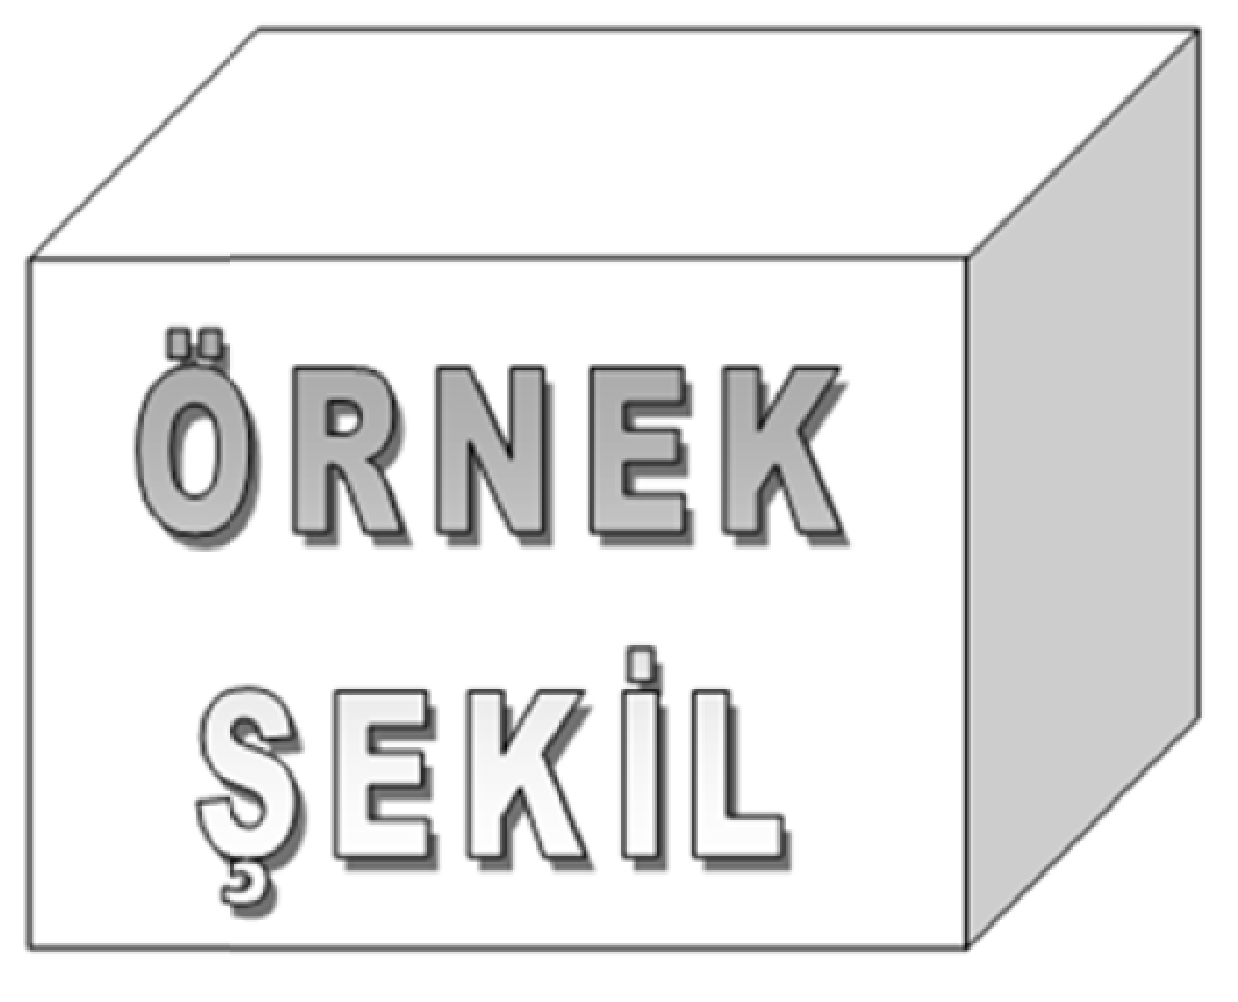
\includegraphics[width=10cm,keepaspectratio=true]{./fig/sekil1}
	% sekil1.eps: 0x0 pixel, 300dpi, 0.00x0.00 cm, bb=14 14 592 479
	\caption{Model structures.}
\end{figure}

\section{Hypothesis}

Lorem ipsum dolor sit amet, consectetur adipiscing elit. Praesent imperdiet, nisi 
nec aliquam cursus, dui turpis mollis nisl, ac consequat tellus sapien sit amet 
magna. Duis vel venenatis velit. Vestibulum ante ipsum primis in faucibus orci 
luctus et ultrices posuere cubilia Curae; Proin malesuada risus nec metus dapibus 
eu tincidunt lectus dignissim. 

Lorem ipsum dolor sit amet, consectetur adipiscing elit. Praesent imperdiet, nisi 
nec aliquam cursus, dui turpis mollis nisl, ac consequat tellus sapien sit amet 
magna. Duis vel venenatis velit. Vestibulum ante ipsum primis in faucibus orci 
luctus et ultrices posuere cubilia Curae; Proin malesuada risus nec metus dapibus 
eu tincidunt lectus dignissim. 

Lorem ipsum dolor sit amet, consectetur adipiscing elit \cite{harper2007}. Praesent imperdiet, nisi 
nec aliquam cursus, dui turpis mollis nisl, ac consequat tellus sapien sit amet 
magna. Duis vel venenatis velit. Vestibulum ante ipsum primis in faucibus orci 
luctus et ultrices posuere cubilia Curae; Proin malesuada risus nec metus dapibus 
eu tincidunt lectus dignissim \cite{unesco}.

Lorem ipsum dolor sit amet, consectetur adipiscing elit. Praesent imperdiet, nisi 
nec aliquam cursus, dui turpis mollis nisl, ac consequat tellus sapien sit amet 
magna. Duis vel venenatis velit. Vestibulum ante ipsum primis in faucibus orci 
luctus et ultrices posuere cubilia Curae; Proin malesuada risus nec metus dapibus 
eu tincidunt lectus dignissim.Lorem ipsum dolor sit amet, consectetur adipiscing elit. 
Praesent imperdiet, nisi nec aliquam cursus, dui turpis mollis nisl, ac consequat 
tellus \cite{mccaffrey88} \cite{moore91} \cite{nelson88}
\cite{sisaky} \cite{simpsondvd} \cite{startrek} \cite{TS-40561} \cite{url-1} \cite{url-2}
\cite{vanden2001}.

Duis vel venenatis velit. Vestibulum ante ipsum primis in faucibus orci 
luctus et ultrices posuere cubilia Curae; Proin malesuada risus nec metus dapibus 
eu tincidunt lectus dignissim.

Lorem ipsum dolor sit amet, consectetur adipiscing elit. Praesent imperdiet, nisi 
nec aliquam cursus, dui turpis mollis nisl, ac consequat tellus sapien sit amet 
magna. Duis vel venenatis velit. Vestibulum ante ipsum primis in faucibus orci 
luctus et ultrices posuere cubilia Curae; Proin malesuada risus nec metus dapibus 
eu tincidunt lectus dignissim.

\begin{table*}
	{\setlength{\tabcolsep}{14pt}
		\caption{Table captions must be ended with a full stop.}
		\begin{center}
			\vspace{-6mm}
			\begin{tabular}{cccc}
				\hline\hline
				Column A & Column B & Column C & Column D \\
				\hline
				Row A & Row A & Row A & Row A \\
				Row B & Row B & Row B & Row B \\
				Row C & Row C & Row C & Row C \\
				\hline
			\end{tabular}
			\vspace{-6mm}
		\end{center}
		\label{sitable3}}
\end{table*}

Lorem ipsum dolor sit amet, consectetur adipiscing elit. Praesent imperdiet, nisi 
nec aliquam cursus, dui turpis mollis nisl, ac consequat tellus sapien sit amet 
magna. Duis vel venenatis velit. Vestibulum ante ipsum primis in faucibus orci 
luctus et ultrices posuere cubilia Curae; Proin malesuada risus nec metus dapibus 
eu tincidunt lectus dignissim \cite{1993JHyd..144..193B}.


                                       
%%%%%%%%%%%%%%%%%%%%%%%%%%%%%%%%%%%%%%%%%%%%%%%%%%%%%%%%%%%%%%%%%
\chapter{TABLES AND FIGURES }\label{Ch2}
%%%%%%%%%%%%%%%%%%%%%%%%%%%%%%%%%%%%%%%%%%%%%%%%%%%%%%%%%%%%%%%%%
\vspace*{-12pt} % If no text above section, use this vspace* to lift the whole part to the proper starting point - SBÖ
\section{Figure Citations and Figure Example}

Tables and figures given in appendices must be numbered with the number of the appendix they are in (i.e. Table \ref{TableA.1}, Table A.2, Figure A.1, Figure A.2).

In tables and figures, font size could be reduced to 8 pt, if necessary.

Tables must be prepared using the same font type as the thesis. The font type used in figures must be consistent throughout the thesis.

Tables and figures must be placed after they are first cited in the main text body, but must be as close as possible, in accordance with the rules in this guideline (Figure \ref{Figure2.1}). All tables and figures must be cited before they are used in the main text body (Table \ref{Table2.1}).

All tables and figures must be horizontally centered on the page.

The numbering of the tables and the figures must be such that the first number is the number of the chapter the table/figure is placed under (for appendices, the letter of the appendix), and the second number is the number of order (i.e. Table \ref{Table2.2}, Figure \ref{Figure2.2}, Table \ref{TableA.1}, Figure \ref{Figure2.3}). The words “Table” and “Figure” and numbers must be bold.

For table numbers and captions, 1 line spacing, 12 pt (before) and 6 pt (after) paragraph spacing must be set. Table captions must be ended with a full stop. A table and its caption must be on the same page. 

Multiple tables/figures could be placed on one page, however, table/figures spanning more than 4 consecutive pages must be given in appendices rather than the main text body.

The first paragraph following a table must have 12 pt (before) and 6 pt (after) paragraph spacing. Titles following a table must have the standard formatting as previously specified. 

Footnotes for a table must be written with 1 line spacing and a font size 2 pt smaller than the main text body. 
For figure numbers and captions, 1 line spacing, 6 pt (before) and 12 pt (after) paragraph spacing must be set. Figure captions must be ended with a full stop. A figure and its caption must be on the same page. 

For figures spanning more than one page, the same number and caption must be written below the continued figure, with the expression ”continued” added in brackets (i.e. \textbf{Table \ref{Table2.1} (continued):} Metal composition of wastes. \textbf{Figure \ref{Figure2.1} (continued):} Water supply network of ISTANBUL.).

Plots, images and musical notes must be numbered and captioned as figures. Musical notes must be written according to the format rules set by the ITU School of Traditional Turkish Music. 

It is recommended that elements that increase the page thickness and disrupt the binding structure of theses such as  folded pages or additional items embedded on pages are given as appendices.

\vspace{6pt}
\begin{figure}[h]
	\centering
	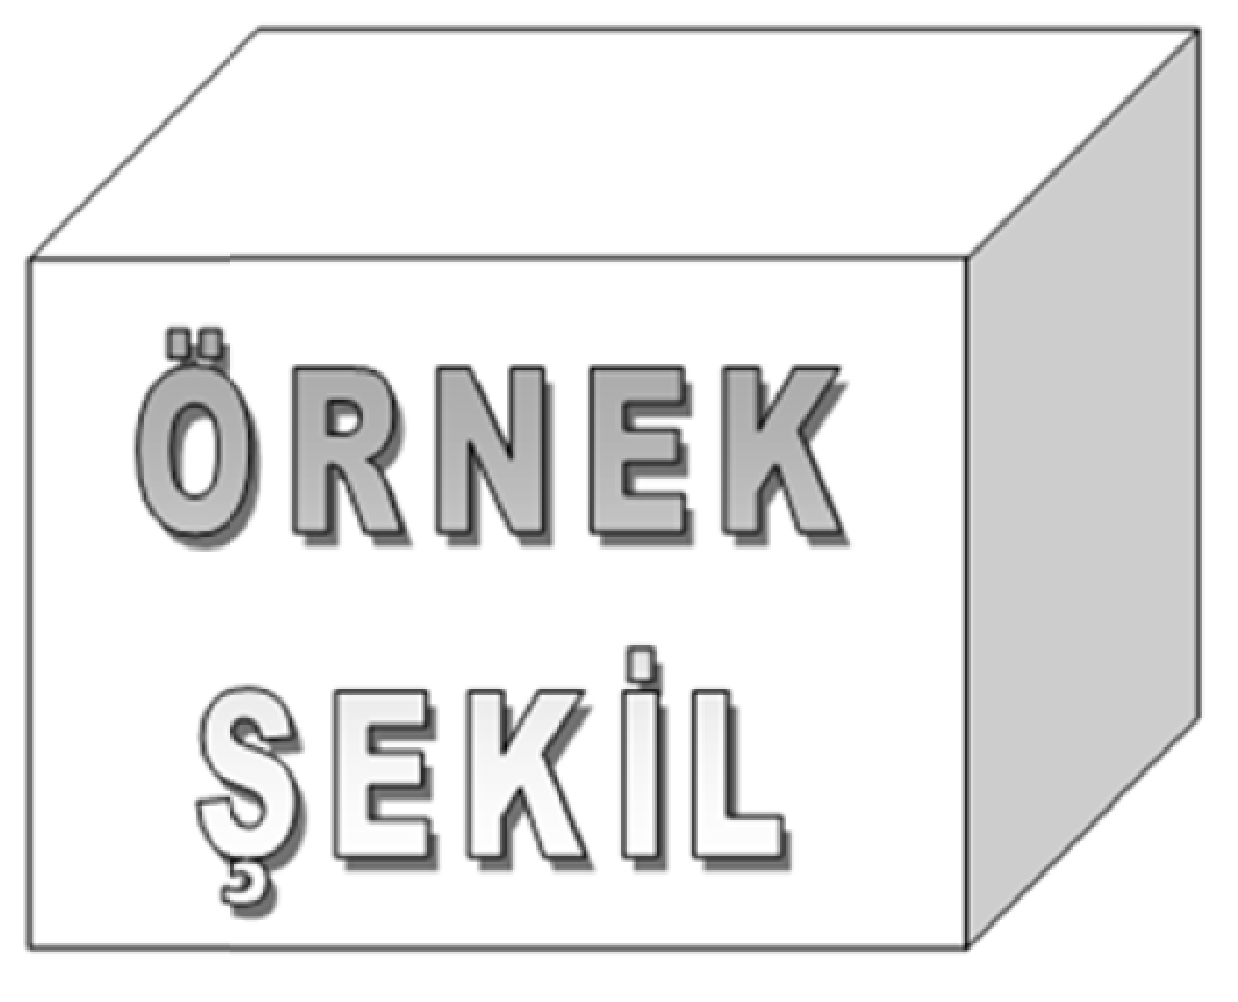
\includegraphics[scale=.3]{./fig/sekil1}
	% sekil1.eps: 0x0 pixel, 300dpi, 0.00x0.00 cm, bb=14 14 592 479
	\vspace{6pt}
	\caption{All tables and figures must be horizontally centered on the page.}
	\label{Figure2.1}
\end{figure}

%\begin{figure}
%	\begin{minipage}[b]{.5\linewidth}
%		\centering
%		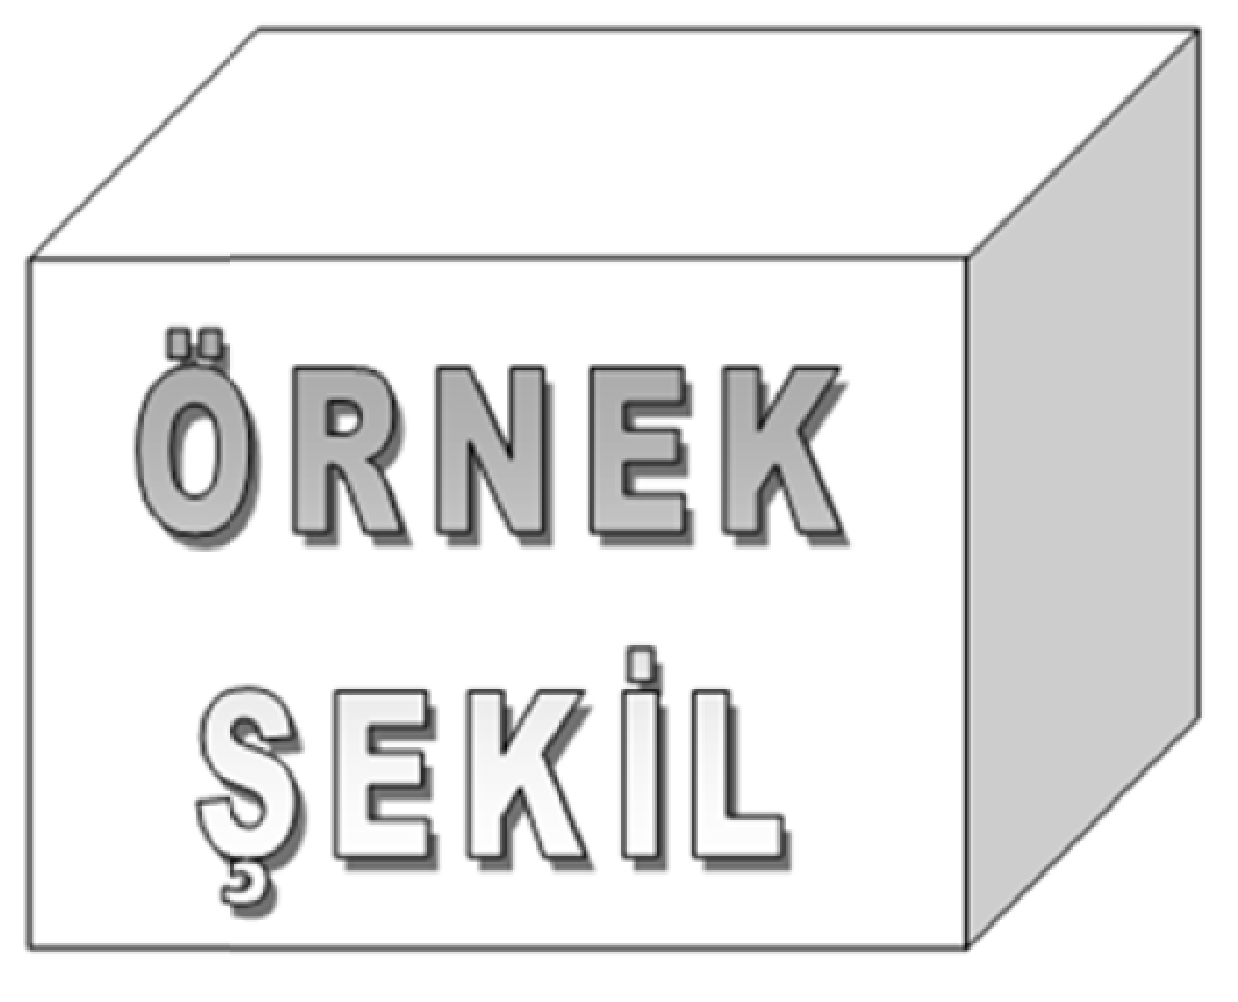
\includegraphics[scale=.2]{./fig/sekil1}
%		\subcaption{A subfigure}\label{Figure2.2a}
%	\end{minipage}
%	\begin{minipage}[b]{.5\linewidth}
%		\centering
%		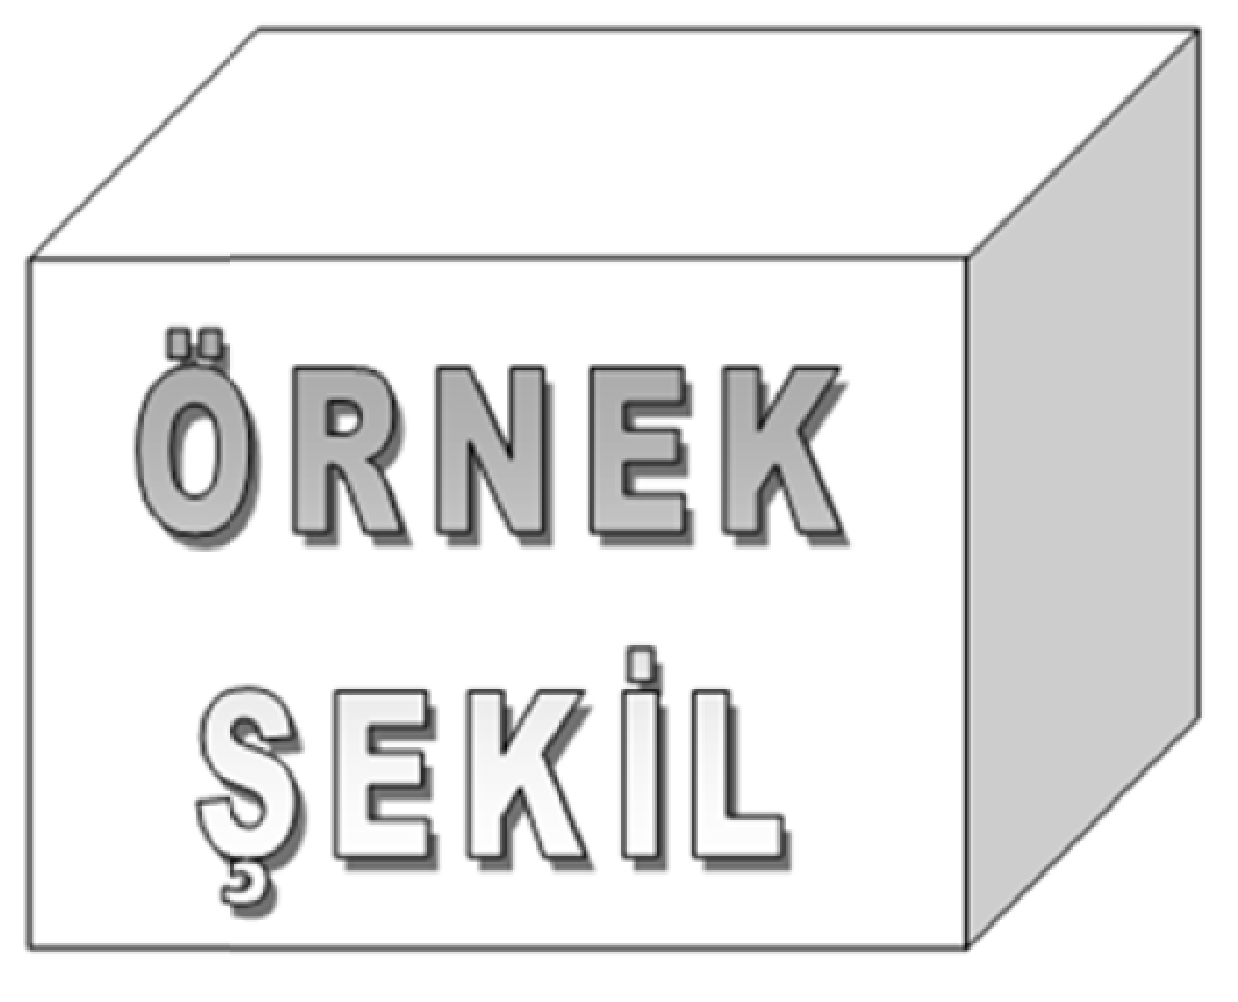
\includegraphics[scale=.2]{./fig/sekil1}
%		\subcaption{Another subfigure}\label{Figure2.2b}
%	\end{minipage}
%	\caption{A figure}\label{Figure2.2} % If no need a caption for main figure comment it out 
%\end{figure}
%%Figure letter: \subref{Figure2.2a}

%\begin{figure}
%	\begin{subfigure}[b]{.5\linewidth}
%		\centering
%		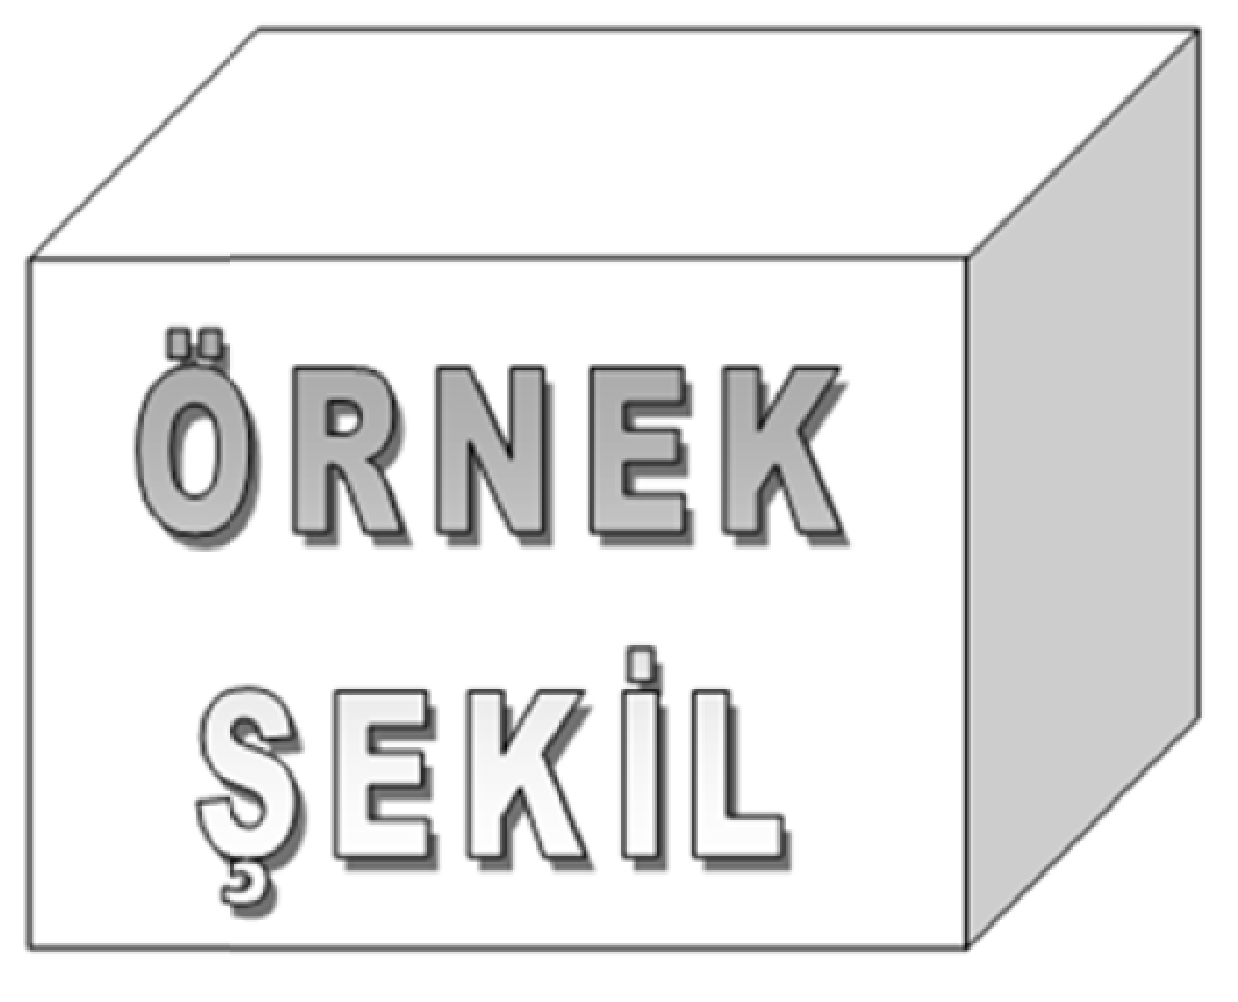
\includegraphics[scale=.2]{./fig/sekil1}
%		\caption{A subfigure}\label{Figure2.3a}
%	\end{subfigure}
%	\begin{subfigure}[b]{.5\linewidth}
%		\centering
%		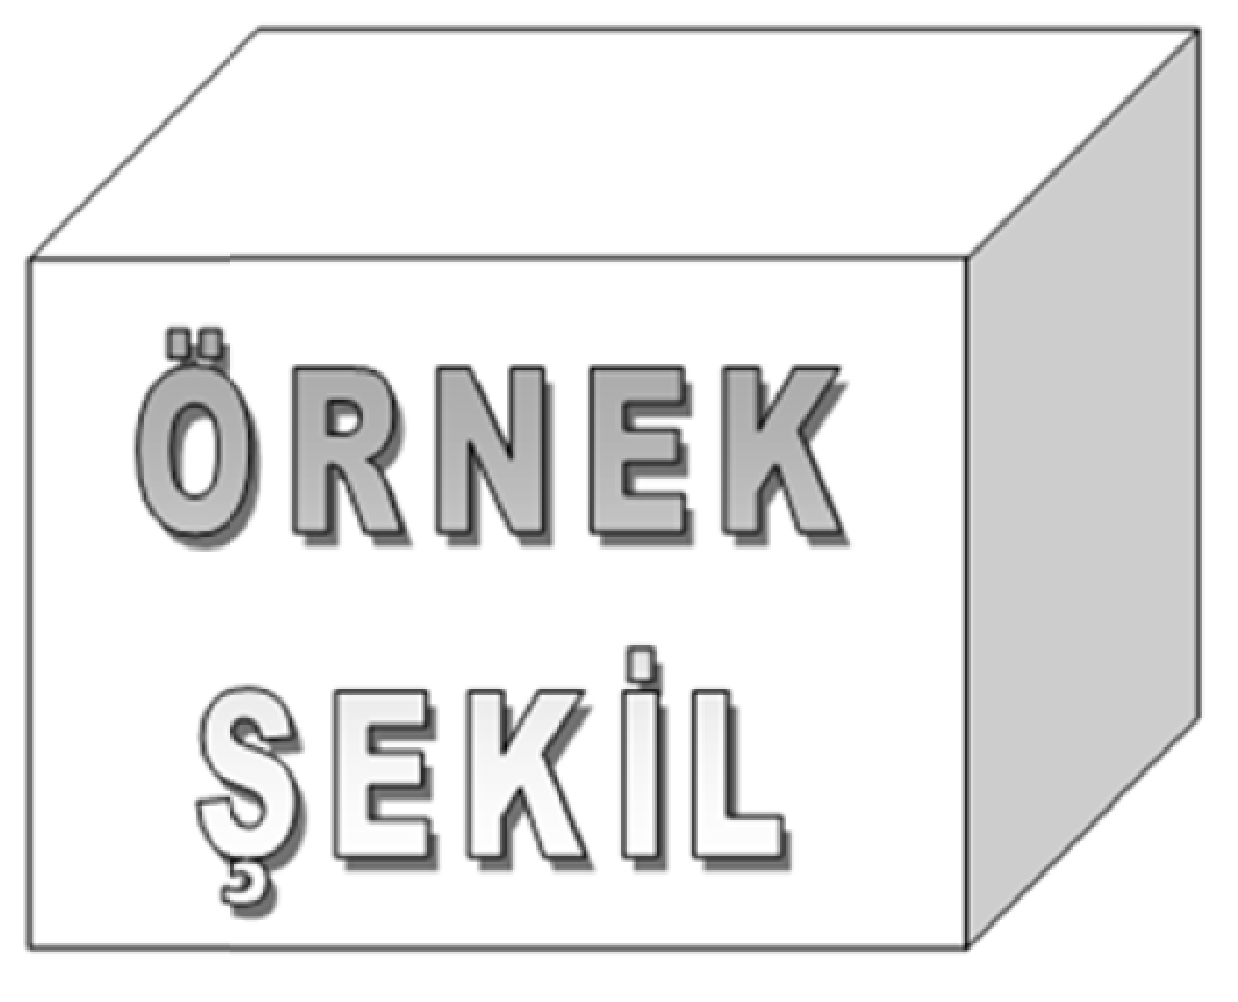
\includegraphics[scale=.2]{./fig/sekil1}
%		\caption{Another subfigure}\label{Figure2.3b}
%	\end{subfigure}
%	\caption{A figure}\label{Figure2.3}
%\end{figure}

% Subfigure example with proper LOF usage - SBÖ
\begin{figure}[h]
	\centering
	\begin{subfigure}{.8\textwidth}
		\centering
		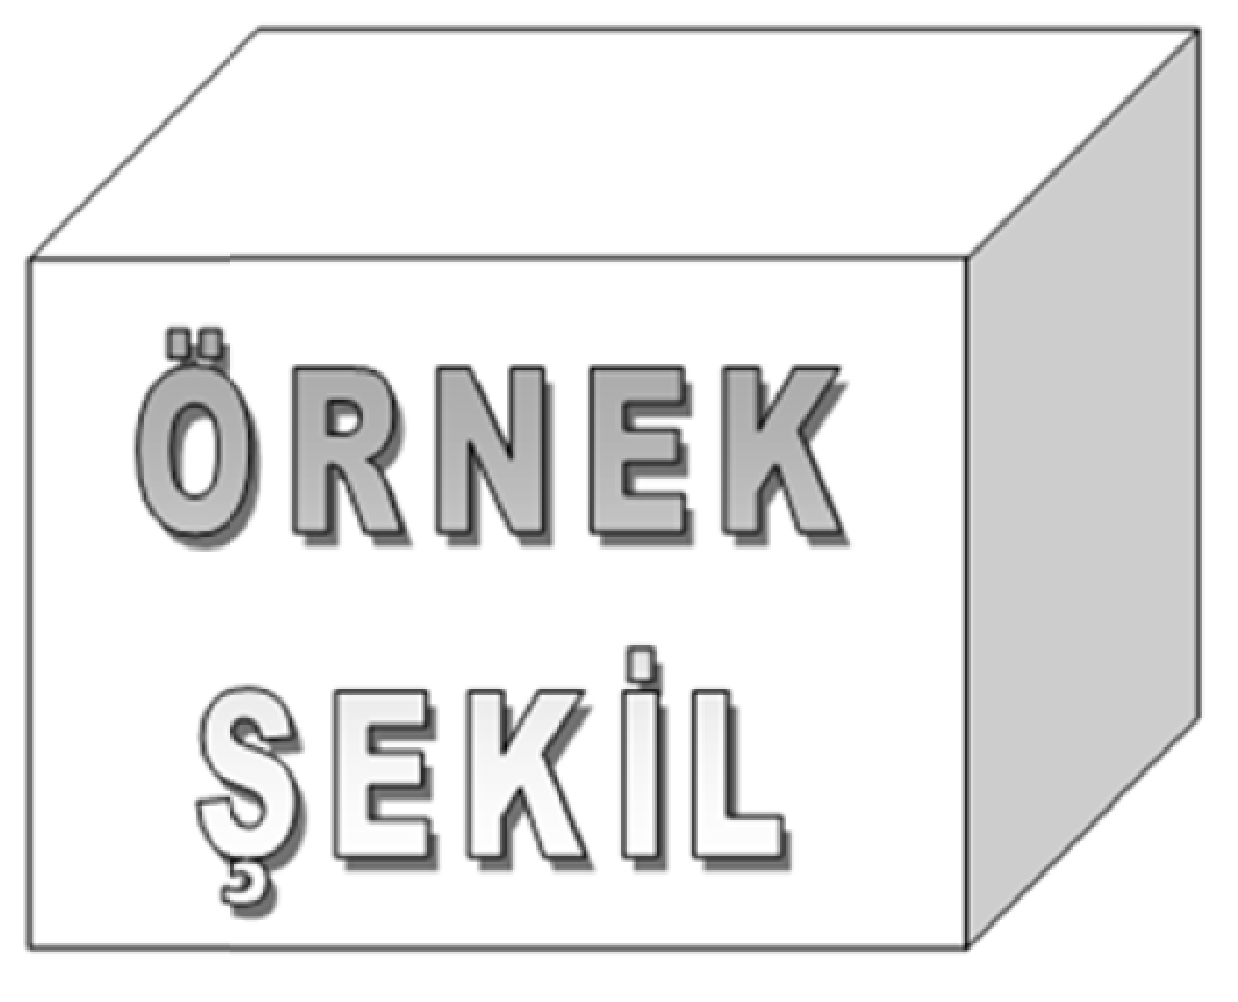
\includegraphics[scale=.3]{./fig/sekil1}
		\firstsubcaption{First subcaption of the subfigure.}
		\label{Figure2.2a}
	\end{subfigure}
	\begin{subfigure}{.8\textwidth}
		\centering
		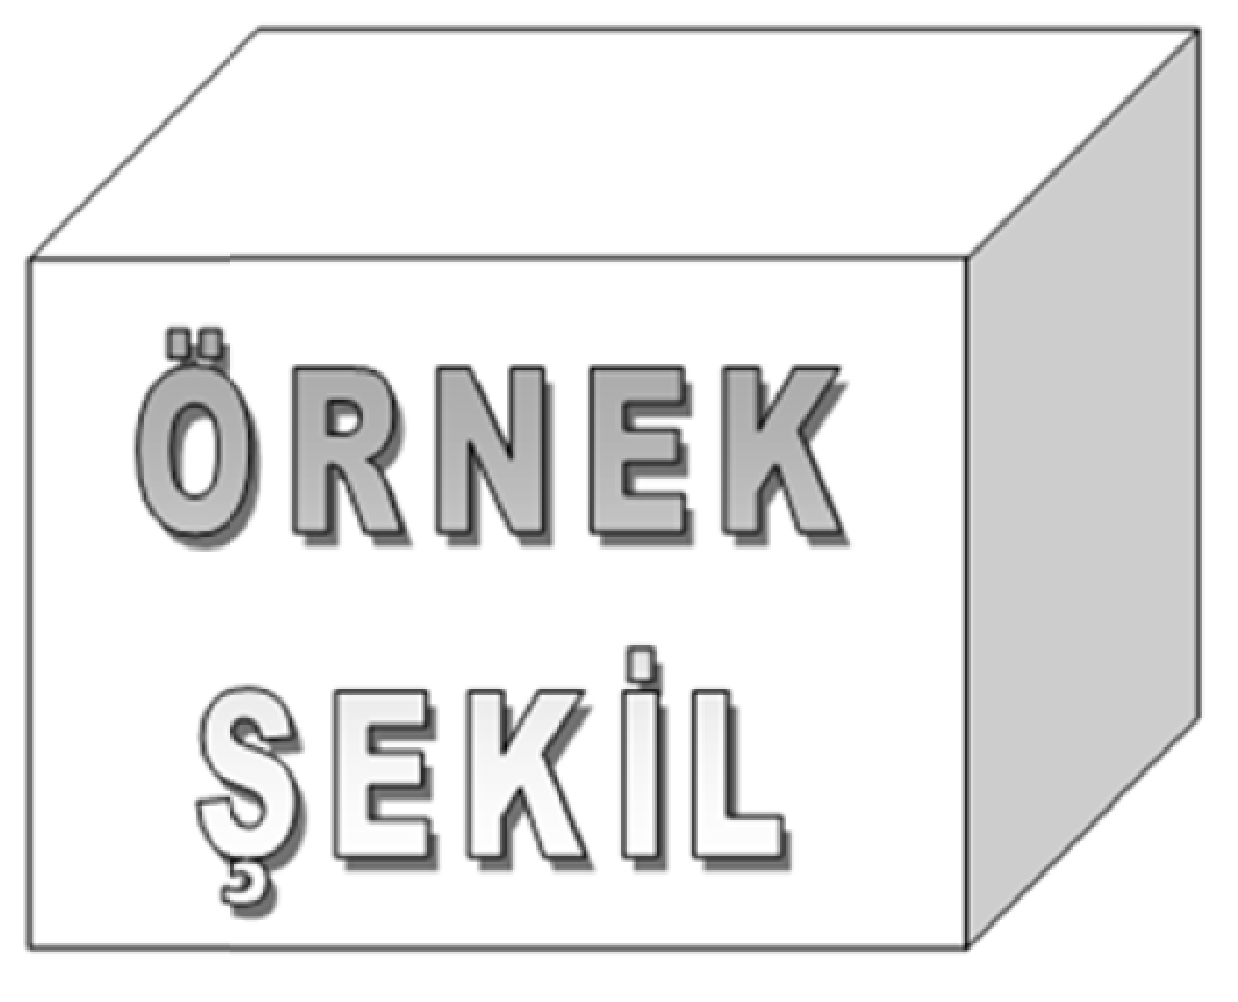
\includegraphics[scale=.3]{./fig/sekil1}
		\nextsubcaption{Second subcaption of the subfigure.}
		\label{Figure2.2b}
	\end{subfigure}
    \caption{An example of subfigure main caption.}\label{Figure2.2}
\end{figure}

%\begin{figure}
%	\centering     % not \center
%	\subcaption[]{Another subfigure}{\label{fig:a}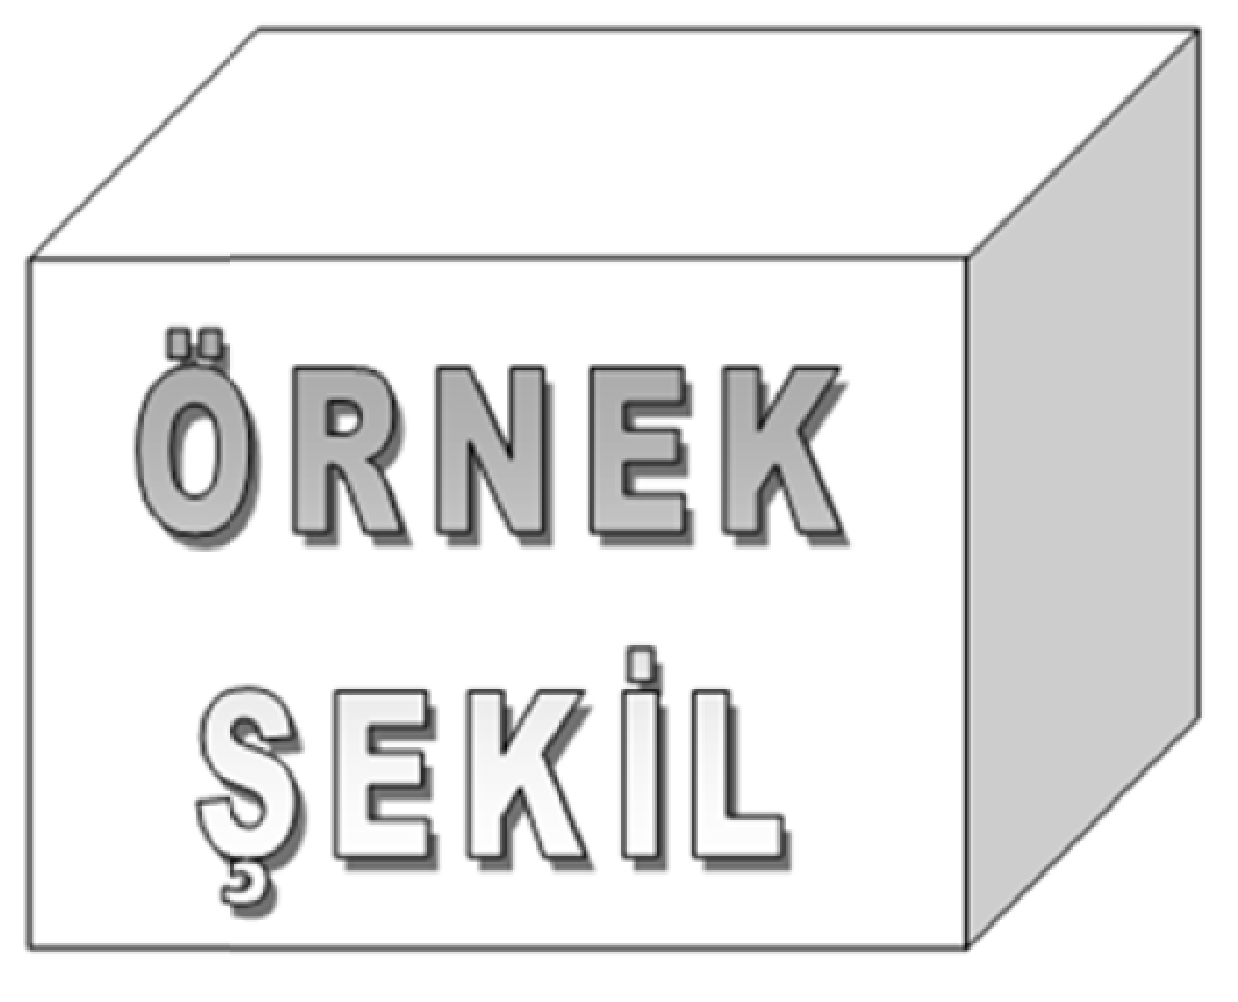
\includegraphics[scale=.2]{./fig/sekil1}}
%	\subcaption[]{Another subfigure}{\label{fig:b}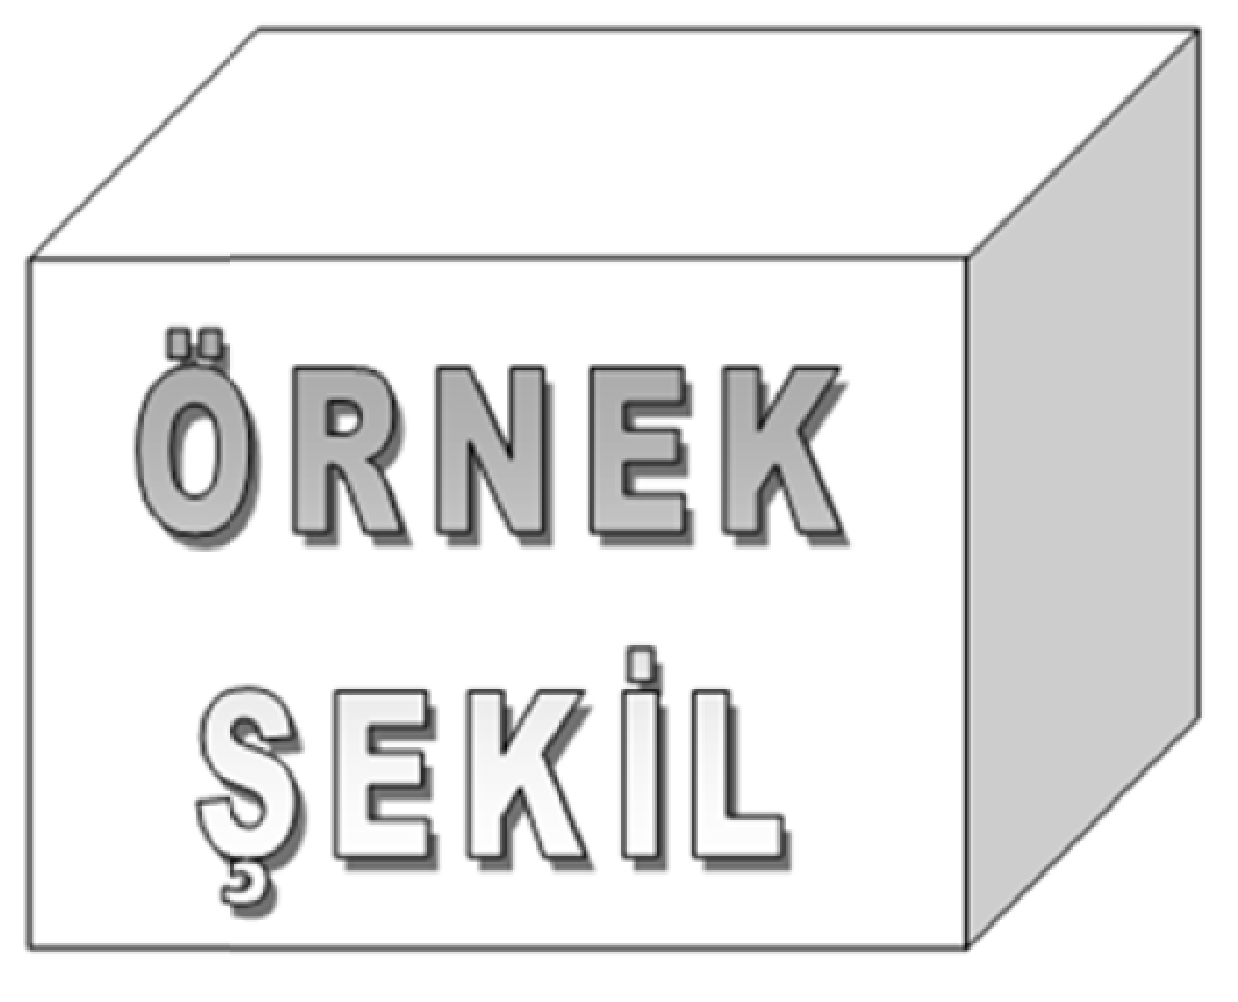
\includegraphics[scale=.2]{./fig/sekil1}}
%	%\caption{(a) this is fig 1 (b) this is fig 2.}
%	\label{L50}
%\end{figure}

In Figure \ref{Figure2.2}, sed diam nonumy eirmod tempor invidunt ut labore et dolore magna aliquyam erat, sed diam voluptua. At vero eos et accusam et justo duo dolores et ea rebum. Lorem ipsum dolor sit amet, consetetur sadipscing elitr, sed diam nonumy eirmod tempor invidunt ut labore et dolore magna aliquyam erat, sed diam voluptua. At vero eos et accusam et justo duo dolores et ea rebum. At vero eos et accusam et justo duo dolores et ea rebum. At vero eos et accusam et justo duo dolores et ea rebum. At vero eos et accusam et justo duo dolores et ea rebum. At vero eos et accusam et justo duo dolores et ea rebum. At vero eos et accusam et justo duo dolores et ea rebum. At vero eos et accusam et justo duo dolores et ea rebum in Figure \ref{Figure2.2a}.

\begin{figure}
	\centering
	
\includegraphics[width=10cm,keepaspectratio=true]{./fig/sekil2}
	% sekil2.eps: 0x0 pixel, 300dpi, 0.00x0.00 cm, bb=14 14 818 556
	\vspace{3pt}
	\caption{Example figure.}
	\label{Figure2.3}
\end{figure}
\vspace{-6pt}
\section{Landscape-oriented, full-page figure}

Lorem ipsum dolor sit amet, consetetur sadipscing elitr, sed diam nonumy eirmod tempor invidunt ut labore et dolore magna aliquyam erat, sed diam voluptua. At vero eos et accusam et justo duo dolores et ea rebum (Figure \ref{Figure2.3}). Lorem ipsum dolor sit amet, consetetur sadipscing elitr, sed diam nonumy eirmod tempor invidunt ut labore et dolore magna aliquyam erat, sed diam voluptua. At vero eos et accusam et justo duo dolores et ea rebum. 

Lorem ipsum dolor sit amet, consetetur sadipscing elitr, sed diam nonumy eirmod tempor invidunt ut labore et dolore magna aliquyam erat, sed diam voluptua. At vero eos et accusam et justo duo dolores et ea rebum. Lorem ipsum dolor sit amet, consetetur sadipscing elitr, sed diam nonumy eirmod tempor invidunt ut labore et dolore magna aliquyam erat, sed diam voluptua. At vero eos et accusam et justo duo dolores et ea rebum. Lorem ipsum dolor sit amet, consetetur sadipscing elitr, sed diam nonumy eirmod tempor invidunt ut labore et dolore magna aliquyam erat, sed diam voluptua. At vero eos et accusam et justo duo dolores et ea rebum \cite{Deci_Ryan_1990}. 

Lorem ipsum dolor sit amet, consetetur sadipscing elitr, sed diam nonumy eirmod tempor invidunt ut labore et dolore magna aliquyam erat, sed diam voluptua. At vero eos et accusam et justo duo dolores et ea rebum. Lorem ipsum dolor sit amet, consetetur sadipscing elitr, sed diam nonumy eirmod tempor invidunt ut labore et dolore magna aliquyam erat, sed diam voluptua. At vero eos et accusam et justo duo dolores et ea rebum. Lorem ipsum dolor sit amet, consetetur sadipscing elitr, sed diam nonumy eirmod tempor invidunt ut labore et dolore magna aliquyam erat, sed diam voluptua. At vero eos et accusam et justo duo dolores et ea rebum. Lorem ipsum dolor sit amet, consetetur sadipscing elitr, sed diam nonumy eirmod tempor invidunt ut labore et dolore magna aliquyam erat, sed diam voluptua. At vero eos et accusam et justo duo dolores et ea rebum \cite{lepichon}.

% Change margins on the fly to reset the page margins to one inch - SBÖ
\newenvironment{changemargin}[4]{
	\begin{list}{}{
			\setlength{\voffset}{#1}
			\setlength{\oddsidemargin}{#2}
			\setlength{\evensidemargin}{#3}
			\setlength{\textheight}{#3}
		}
		\item[] ~ \par
		% Get rid of the extra space inserted by the previous line
		%\vspace*{-2em}
	}{
	\end{list}
}

% All the figures and also odd page figures normally face inside the thesis, however the rule requires figures always face to the right. - SBÖ
% Figures on landscape pages has to be centered and facing to the right (ITU) - SBÖ
\begin{landscape}
	\thispagestyle{empty} %Remove the bottom page numbering
%	\begin{changemargin}{-0.4mm}{0mm}{0mm} %Set all the margins to zero - SBÖ
	%\thispagestyle{lscape}
	\vspace*{5mm}
	\begin{figure*}[ht]
		\centering
		%\begin{tabular}{@{}cc@{}}
		
\includegraphics[scale=.41,keepaspectratio=true]{./fig/sekil3} %&
		%
\includegraphics[width=50mm]{./fig/sekil3}
		%\end{tabular}                                       
		\caption{Landscape-oriented, full-page figure.}
		\label{Figure2.4}
	\end{figure*}
	
% Set the page number on the right side for odd numbered pages
      \begin{tikzpicture}[remember picture, overlay]
		\node[xshift=-25mm+148.5mm, yshift=17mm-210mm+22mm] (number) at (current page text area.east) {\thepage};
	  \end{tikzpicture}
	  
%\end{changemargin}
\end{landscape}

% All the figures and also even page figures normally face inside the thesis, however the rule requires figures always face to the right. - SBÖ
% Figures on landscape pages has to be centered and facing to the right (ITU) - SBÖ
\begin{landscape}
	\thispagestyle{empty} % Remove the bottom page numbering
%	\begin{changemargin}{-0.4mm}{0mm}{0mm} %Set all the margins to zero - SBÖ
		%\thispagestyle{lscape}

		\vspace*{20mm}
		\begin{figure*}[ht]
			\centering
			%\begin{tabular}{@{}cc@{}}
				
\includegraphics[scale=.41,keepaspectratio=true]{./fig/sekil3} %&
				%
\includegraphics[width=50mm]{./fig/sekil3}
			%\end{tabular}                                       
			\caption{Landscape-oriented, full-page figure.}
			\label{Figure2.5}
		\end{figure*}
	   
% Set the page number on the left side for even numbered pages
		%\begin{tikzpicture}[remember picture, overlay]
		% \node[xshift=-25mm+148.5mm, yshift=-1mm-15mm, rotate=180] (number) at (current page text area.east) {\thepage};
		%\end{tikzpicture}
		
% Set the page number on the right side for even numbered pages as well
		\begin{tikzpicture}[remember picture, overlay]
		 \node[xshift=-25mm+148.5mm, yshift=17mm-210mm+22mm] (number) at (current page text area.east) {\thepage};
		\end{tikzpicture}
		
%	\end{changemargin}
\end{landscape}

%\newpage
\section{Table Citations and Table Example}

Lorem ipsum dolor sit amet, consetetur sadipscing elitr, sed diam nonumy eirmod tempor invidunt ut labore et dolore magna aliquyam erat, sed diam voluptua. At vero eos et accusam et justo duo dolores et ea rebum. Stet clita kasd gub rgren, no sea takimata sanctus est Lorem ipsum dolor sit amet, consetetur sadipscing elitr, sed diam nonumy eirmod tempor invidunt ut lab ore sit et dolore magna.

\begin{table*}[h]
	{\setlength{\tabcolsep}{14pt}
		\caption{Table with single row and centered columns.}
		\begin{center}
			\vspace{-6mm}
			\begin{tabular}{cccc}
				\hline \\[-2.45ex] \hline \\[-2.1ex]
				Column A & Column B & Column C & Column D \\
				\hline \\[-1.8ex]
				Row A & Row A & Row A & Row A \\
				Row B & Row B & Row B & Row B \\
				Row C & Row C & Row C & Row C \\
				\hline
			\end{tabular}
			\vspace{-6mm}
		\end{center}
		\label{Table2.1}}
\end{table*}

As seen in Table \ref{Table2.1}, lorem ipsum dolor sit amet, consetetur sadipscing elitr, sed diam nonumy eirmod tempor invidunt ut labore et dolore magna aliquyam erat, sed diam voluptua. At vero eos et accusam et justo duo dolores et ea rebum. Stet clita kasd gub rgren, no sea takimata sanctus est Lorem ipsum dolor sit amet, consetetur sadipscing elitr, sed diam nonumy eirmod tempor invidunt ut lab ore sit et dolore magna.

\begin{table*}[h]
	{\setlength{\tabcolsep}{14pt}
		\caption{Table captions must be ended with a full stop.}
		\begin{center}
			\vspace{-6mm}
			\begin{tabular}{cccc}
				\hline \\[-2.45ex] \hline \\[-2.1ex]
				Column A & Column B & Column C & Column D \\
				\hline \\[-1.8ex]
				Row A & Row A & Row A & Row A \\
				Row B & Row B & Row B & Row B \\
				Row C & Row C & Row C & Row C \\
				\hline
			\end{tabular}
			\vspace{-6mm}
		\end{center}
		\label{Table2.2}}
\end{table*}

Lorem ipsum dolor sit amet, consetetur sadipscing elitr, sed diam nonumy eirmod tempor invidunt ut labore et dolore magna aliquyam erat, sed diam voluptua. At vero eos et accusam et justo duo dolores et ea rebum, as seen in Table \ref{Table2.2}. 

Lorem ipsum dolor sit amet, consetetur sadipscing elitr, sed diam nonumy eirmod tempor invidunt ut labore et dolore magna aliquyam erat, sed diam voluptua. At vero eos et accusam et justo duo dolores et ea rebum. Stet clita kasd gub rgren, no sea takimata sanctus est Lorem ipsum dolor sit amet, consetetur sadipscing elitr, sed diam nonumy eirmod tempor invidunt ut lab ore sit et dolore magna. Lorem ipsum dolor sit amet, consetetur sadipscing elitr, sed diam nonumy eirmod tempor invidunt ut labore et dolore magna aliquyam erat, sed diam voluptua. At vero eos et accusam et justo duo dolores et ea rebum \cite{Roberts_Jackson_1991}. 

\section{Landscape-oriented, full-page table}

Lorem ipsum dolor sit amet, consetetur sadipscing elitr, sed diam nonumy eirmod tempor invidunt ut labore et dolore magna aliquyam erat, sed diam voluptua. At vero eos et accusam et justo duo dolores et ea rebum. Stet clita kasd gub rgren, no sea takimata sanctus est Lorem ipsum dolor sit amet, consetetur sadipscing elitr, sed diam nonumy eirmod tempor invidunt ut lab ore sit et dolore magna.

% ---------------------------------------------------------------- %
% Page numbers must be on the bottom-middle of short side (when    %
% portrait-oriented), or bottom-middle of long side (when	       %
% landscape-oriented)						                       %
% ---------------------------------------------------------------- %
% Odd page landscape table and page numbering - SBÖ		
\begin{landscape}
	\thispagestyle{empty}
%	\vspace*{-6mm}
%	\begin{changemargin}{0.4mm}{0mm}{0mm} %Set all the margins to zero - SBÖ
	\begin{table*}[htb!]
		{\setlength{\tabcolsep}{14pt}
			%\hspace*{5mm}
			%\vspace*{-6mm}
			\caption{Prof. Dr. Galip TEPEHAN \,\, Captioning in landscape-oriented pages:
				the most important aspect is to align the lines horizontally.}
			\begin{center}
				\vspace{-6mm}
				\begin{tabular}{lccrrrrr}
					\hline\hline
					\multirow{2}{*}{Parametre} & \multirow{2}{*}{Column 2} & \multirow{2}{*}{Column 3} & \multicolumn{3}{c|}{Column 4} & \multicolumn{2}{c}{Column 5}\\ \cline{4-8}
					& & & Subcolumn & Subcolumn & Subcolumn & Subcolumn & Subcolumn\\
					\hline
					Row 1 & -7.680442 & 7.6986348 & 0.00 & 0.00 & 0.00 & 12 & 12 \\
					Row 2 & 140 & - & 0.50 & 0.00 & 0.00 & 0 & 0 \\
					Row 3 & 37.174357 & 37.16192697 & 0.00 & 0.00 & 0.00 & 0 & 24 \\
					Row 4 & 140 & - & 0.50 & 0.00 & 0.00 & 0 & 0 \\
					Row 5 & 37.174357 & 37.16192697 & 0.00 & 0.00 & 0.00 & 0 & 24 \\
					Row 6 & 140 & - & 0.50 & 0.00 & 0.00 & 0 & 0 \\
					Row 7 & 37.174357 & 37.16192697 & 0.00 & 0.00 & 0.00 & 0 & 24 \\
					Row 8 & 140 & - & 0.50 & 0.00 & 0.00 & 0 & 0 \\
					Row 9 & 37.174357 & 37.16192697 & 0.00 & 0.00 & 0.00 & 0 & 24 \\
					Row 10 & 140 & - & 0.50 & 0.00 & 0.00 & 0 & 0 \\
					Row 11 & 37.174357 & 37.16192697 & 0.00 & 0.00 & 0.00 & 0 & 24 \\
					Row 12 & 140 & - & 0.50 & 0.00 & 0.00 & 0 & 0 \\
					Row 13 & 37.174357 & 37.16192697 & 0.00 & 0.00 & 0.00 & 0 & 24 \\
					Row 14 & 140 & - & 0.50 & 0.00 & 0.00 & 0 & 0 \\
					Row 15 & 37.174357 & 37.16192697 & 0.00 & 0.00 & 0.00 & 0 & 24 \\
					\hline
				\end{tabular}
			\end{center}
			\begin{center}
				\label{Table2.3}
			\end{center}
		}
	\end{table*}
% Set the page number on the right side for odd numbered pages
		\begin{tikzpicture}[remember picture,overlay]
		\node[xshift=-10mm+148.5mm, yshift=2mm-210mm+37mm] (number) at (current page text area.east) {\thepage};
		\end{tikzpicture}
%   \end{changemargin}
\end{landscape}

% ---------------------------------------------------------------- %
% Page numbers must be on the bottom-middle of short side (when    %
% portrait-oriented), or bottom-middle of long side (when	       %
% landscape-oriented)						                       %
% ---------------------------------------------------------------- %
% Even page landscape table and page numbering - SBÖ		
\begin{landscape}
	\thispagestyle{empty}
	%\vspace*{-6mm}
%	\begin{changemargin}{0.4mm}{0mm}{0mm} %Set all the margins to zero - SBÖ
		\begin{table*}[htb!]
			{\setlength{\tabcolsep}{14pt}
				%\hspace*{5mm}
				%\vspace*{-6mm}
				\caption{Prof. Dr. Galip TEPEHAN \,\, Captioning in landscape-oriented pages:
					the most important aspect is to align the lines horizontally.}
				\begin{center}
					\vspace{-6mm}
					\begin{tabular}{lccrrrrr}
						\hline\hline
						\multirow{2}{*}{Parametre} & \multirow{2}{*}{Column 2} & \multirow{2}{*}{Column 3} & \multicolumn{3}{c|}{Column 4} & \multicolumn{2}{c}{Column 5}\\ \cline{4-8}
						& & & Subcolumn & Subcolumn & Subcolumn & Subcolumn & Subcolumn\\
						\hline
						Row 1 & -7.680442 & 7.6986348 & 0.00 & 0.00 & 0.00 & 12 & 12 \\
						Row 2 & 140 & - & 0.50 & 0.00 & 0.00 & 0 & 0 \\
						Row 3 & 37.174357 & 37.16192697 & 0.00 & 0.00 & 0.00 & 0 & 24 \\
						Row 4 & 140 & - & 0.50 & 0.00 & 0.00 & 0 & 0 \\
						Row 5 & 37.174357 & 37.16192697 & 0.00 & 0.00 & 0.00 & 0 & 24 \\
						Row 6 & 140 & - & 0.50 & 0.00 & 0.00 & 0 & 0 \\
						Row 7 & 37.174357 & 37.16192697 & 0.00 & 0.00 & 0.00 & 0 & 24 \\
						Row 8 & 140 & - & 0.50 & 0.00 & 0.00 & 0 & 0 \\
					\end{tabular}
				\end{center}
				\begin{center}
					\label{Table2.4}
				\end{center}
			}
		\end{table*}
% Set the page number on the right side for even numbered pages
		\begin{tikzpicture}[remember picture,overlay]
		\node[xshift=-25mm+148.5mm, yshift=2mm-210mm+37mm] (number) at (current page text area.east) {\thepage};
		\end{tikzpicture}
%	\end{changemargin}
\end{landscape}

\begin{table}[!htbp] \centering
	\caption{ Neighborhoods Visited }
	\vspace{-3mm}
	\label{}
	\begin{tabular}{@{\extracolsep{5pt}} llrrr} 
	\\[-1.8ex]\hline 
		\hline \\[-1.8ex] 
		\multicolumn{1}{c}{Variable} & \multicolumn{1}{c}{Values} & \multicolumn{1}{c}{Count} & \multicolumn{1}{c}{\%} & \multicolumn{1}{c}{Cum. \%} \\
		\hline \\[-1.8ex] 
		\multirow{ 4 }{*}{ visit }  &  FALSE  &  2  &  33.33  &  33.33  \\
		\hhline{}  &  TRUE  &  3  &  50.00  &  83.33  \\
		\hhline{}  &  NA  &  1  &  16.67  &  100.00  \\
	    \hhline{}  &  Total  &  6  &  100.00  &    \\
		\hline \\[-1.8ex] 
	\end{tabular}
\end{table}

% Multi-page longtable example spreading couple of pages - SBÖ
\begin{center}
	\begin{longtable}{ccc}
		%Here is the caption, the stuff in [] is the table of contents entry,
		%the stuff in {} is the title that will appear on the first page of the
		%table.
		\caption[Feasible triples for a highly variable Grid]{Feasible triples
			for highly variable Grid, MLMMH.} \label{Table2.6} \vspace{-1.75mm}\\
		%This is the header for the first page of the table...
		\hline\\[-2.45ex] \hline \\[-1.8ex] % Distancing of the hlines adjausted from the text 
		\multicolumn{1}{c}{{Time (s)}} &
		\multicolumn{1}{c}{{Triple chosen}} &
		\multicolumn{1}{c}{{Other feasible triples}} \\[0.5ex] \hline
		\\[-1.8ex]
		\endfirsthead
		
		%This is the header for the remaining page(s) of the table...
		\multicolumn{3}{c}{{\tablename} \textbf{\thetable{}} \textbf{(continued) :} Feasible triples
			for highly variable Grid, MLMMH.} \\[0.5ex]
		\hline\\[-2.45ex] \hline \\[-1.8ex]
		\multicolumn{1}{c}{{Time (s)}} &
		\multicolumn{1}{c}{{Triple chosen}} &
		\multicolumn{1}{c}{{Other feasible triples}} \\[0.5ex] \hline
		\\[-1.8ex]
		\endhead
		
		%This is the footer for all pages except the last page of the table...
		%\multicolumn{3}{l}{{Continued on Next Page\ldots}} \\
		\\[-1.8ex] \hline
		\endfoot
		
		%This is the footer for the last page of the table...
		\\[-1.8ex] \hline
		\endlastfoot
		
		%Now the data...
		0      & (1, 11, 13725) & (1, 12, 10980), (1, 13, 8235), (2, 2, 0), (3, 1, 0) \\
		2745   & (1, 12, 10980) & (1, 13, 8235), (2, 2, 0), (2, 3, 0), (3, 1, 0) \\
		5490   & (1, 12, 13725) & (2, 2, 2745), (2, 3, 0), (3, 1, 0) \\
		8235   & (1, 12, 16470) & (1, 13, 13725), (2, 2, 2745), (2, 3, 0), (3, 1, 0) \\
		% <data removed>
		164700 & (1, 13, 13725) & (2, 2, 2745), (2, 3, 0), (3, 1, 0) \\
		0      & (1, 11, 13725) & (1, 12, 10980), (1, 13, 8235), (2, 2, 0), (3, 1, 0) \\
		2745   & (1, 12, 10980) & (1, 13, 8235), (2, 2, 0), (2, 3, 0), (3, 1, 0) \\
		5490   & (1, 12, 13725) & (2, 2, 2745), (2, 3, 0), (3, 1, 0) \\
		8235   & (1, 12, 16470) & (1, 13, 13725), (2, 2, 2745), (2, 3, 0), (3, 1, 0) \\
		% <data removed>
		164700 & (1, 13, 13725) & (2, 2, 2745), (2, 3, 0), (3, 1, 0) \\
		0      & (1, 11, 13725) & (1, 12, 10980), (1, 13, 8235), (2, 2, 0), (3, 1, 0) \\
		2745   & (1, 12, 10980) & (1, 13, 8235), (2, 2, 0), (2, 3, 0), (3, 1, 0) \\
		5490   & (1, 12, 13725) & (2, 2, 2745), (2, 3, 0), (3, 1, 0) \\
		8235   & (1, 12, 16470) & (1, 13, 13725), (2, 2, 2745), (2, 3, 0), (3, 1, 0) \\
		% <data removed>
		164700 & (1, 13, 13725) & (2, 2, 2745), (2, 3, 0), (3, 1, 0) \\
		0      & (1, 11, 13725) & (1, 12, 10980), (1, 13, 8235), (2, 2, 0), (3, 1, 0) \\
		2745   & (1, 12, 10980) & (1, 13, 8235), (2, 2, 0), (2, 3, 0), (3, 1, 0) \\
		5490   & (1, 12, 13725) & (2, 2, 2745), (2, 3, 0), (3, 1, 0) \\
		8235   & (1, 12, 16470) & (1, 13, 13725), (2, 2, 2745), (2, 3, 0), (3, 1, 0) \\
		% <data removed>
		164700 & (1, 13, 13725) & (2, 2, 2745), (2, 3, 0), (3, 1, 0) \\
		0      & (1, 11, 13725) & (1, 12, 10980), (1, 13, 8235), (2, 2, 0), (3, 1, 0) \\
		2745   & (1, 12, 10980) & (1, 13, 8235), (2, 2, 0), (2, 3, 0), (3, 1, 0) \\
		5490   & (1, 12, 13725) & (2, 2, 2745), (2, 3, 0), (3, 1, 0) \\
		8235   & (1, 12, 16470) & (1, 13, 13725), (2, 2, 2745), (2, 3, 0), (3, 1, 0) \\
		% <data removed>
		164700 & (1, 13, 13725) & (2, 2, 2745), (2, 3, 0), (3, 1, 0) \\
		0      & (1, 11, 13725) & (1, 12, 10980), (1, 13, 8235), (2, 2, 0), (3, 1, 0) \\
		2745   & (1, 12, 10980) & (1, 13, 8235), (2, 2, 0), (2, 3, 0), (3, 1, 0) \\
		5490   & (1, 12, 13725) & (2, 2, 2745), (2, 3, 0), (3, 1, 0) \\
		8235   & (1, 12, 16470) & (1, 13, 13725), (2, 2, 2745), (2, 3, 0), (3, 1, 0) \\
		% <data removed>
		164700 & (1, 13, 13725) & (2, 2, 2745), (2, 3, 0), (3, 1, 0) \\
		0      & (1, 11, 13725) & (1, 12, 10980), (1, 13, 8235), (2, 2, 0), (3, 1, 0) \\
		2745   & (1, 12, 10980) & (1, 13, 8235), (2, 2, 0), (2, 3, 0), (3, 1, 0) \\
		5490   & (1, 12, 13725) & (2, 2, 2745), (2, 3, 0), (3, 1, 0) \\
		8235   & (1, 12, 16470) & (1, 13, 13725), (2, 2, 2745), (2, 3, 0), (3, 1, 0) \\ \noalign{\penalty-5000}
		% <data removed>
		164700 & (1, 13, 13725) & (2, 2, 2745), (2, 3, 0), (3, 1, 0) \\
		0      & (1, 11, 13725) & (1, 12, 10980), (1, 13, 8235), (2, 2, 0), (3, 1, 0) \\
		2745   & (1, 12, 10980) & (1, 13, 8235), (2, 2, 0), (2, 3, 0), (3, 1, 0) \\
		5490   & (1, 12, 13725) & (2, 2, 2745), (2, 3, 0), (3, 1, 0) \\
		8235   & (1, 12, 16470) & (1, 13, 13725), (2, 2, 2745), (2, 3, 0), (3, 1, 0) \\
		% <data removed>
		164700 & (1, 13, 13725) & (2, 2, 2745), (2, 3, 0), (3, 1, 0) \\
		0      & (1, 11, 13725) & (1, 12, 10980), (1, 13, 8235), (2, 2, 0), (3, 1, 0) \\
		2745   & (1, 12, 10980) & (1, 13, 8235), (2, 2, 0), (2, 3, 0), (3, 1, 0) \\
		5490   & (1, 12, 13725) & (2, 2, 2745), (2, 3, 0), (3, 1, 0) \\
		8235   & (1, 12, 16470) & (1, 13, 13725), (2, 2, 2745), (2, 3, 0), (3, 1, 0) \\
		% <data removed>
		164700 & (1, 13, 13725) & (2, 2, 2745), (2, 3, 0), (3, 1, 0) \\
		0      & (1, 11, 13725) & (1, 12, 10980), (1, 13, 8235), (2, 2, 0), (3, 1, 0) \\
		2745   & (1, 12, 10980) & (1, 13, 8235), (2, 2, 0), (2, 3, 0), (3, 1, 0) \\
		5490   & (1, 12, 13725) & (2, 2, 2745), (2, 3, 0), (3, 1, 0) \\
		8235   & (1, 12, 16470) & (1, 13, 13725), (2, 2, 2745), (2, 3, 0), (3, 1, 0) \\
		% <data removed>
		164700 & (1, 13, 13725) & (2, 2, 2745), (2, 3, 0), (3, 1, 0) \\
		0      & (1, 11, 13725) & (1, 12, 10980), (1, 13, 8235), (2, 2, 0), (3, 1, 0) \\
		2745   & (1, 12, 10980) & (1, 13, 8235), (2, 2, 0), (2, 3, 0), (3, 1, 0) \\
		5490   & (1, 12, 13725) & (2, 2, 2745), (2, 3, 0), (3, 1, 0) \\
		8235   & (1, 12, 16470) & (1, 13, 13725), (2, 2, 2745), (2, 3, 0), (3, 1, 0) \\
		% <data removed>
		164700 & (1, 13, 13725) & (2, 2, 2745), (2, 3, 0), (3, 1, 0) \\
		0      & (1, 11, 13725) & (1, 12, 10980), (1, 13, 8235), (2, 2, 0), (3, 1, 0) \\
		2745   & (1, 12, 10980) & (1, 13, 8235), (2, 2, 0), (2, 3, 0), (3, 1, 0) \\
		5490   & (1, 12, 13725) & (2, 2, 2745), (2, 3, 0), (3, 1, 0) \\
		8235   & (1, 12, 16470) & (1, 13, 13725), (2, 2, 2745), (2, 3, 0), (3, 1, 0) \\
		% <data removed>
		164700 & (1, 13, 13725) & (2, 2, 2745), (2, 3, 0), (3, 1, 0) \\
		0      & (1, 11, 13725) & (1, 12, 10980), (1, 13, 8235), (2, 2, 0), (3, 1, 0) \\
		2745   & (1, 12, 10980) & (1, 13, 8235), (2, 2, 0), (2, 3, 0), (3, 1, 0) \\
		5490   & (1, 12, 13725) & (2, 2, 2745), (2, 3, 0), (3, 1, 0) \\
		8235   & (1, 12, 16470) & (1, 13, 13725), (2, 2, 2745), (2, 3, 0), (3, 1, 0) \\
	\end{longtable}
\end{center}
%%%%%%%%%%%%%%%%%%%%%%%%%%%%%%%%%%%%%%%%%%%%%%%%%%%%%%%%%%%%%%%%%
\chapter{FLOW PREDICTION}\label{ch:fp}
%%%%%%%%%%%%%%%%%%%%%%%%%%%%%%%%%%%%%%%%%%%%%%%%%%%%%%%%%%%%%%%%%

\section{Purpose}

Lorem ipsum dolor sit amet, consectetur adipiscing elit. Sed ac augue vel dui 
adipiscing placerat et nec metus. Donec bibendum sodales mollis. Cras in lacus 
justo, at vestibulum quam. Sed semper, est sit amet consectetur ornare, leo est 
lacinia velit, adipiscing elementum lectus felis at sem. Aenean hendrerit erat eu 
lacus malesuada at sodales arcu egestas. Maecenas euismod urna ut sem luctus et 
congue metus vulputate. Ut pellentesque, neque eget fringilla elementum, ligula 
massa aliquet lorem, et varius nisi lacus vel diam. Etiam vitae metus sed orci 
rutrum fringilla. Phasellus sed velit quam. Mauris vestibulum, mauris a cursus 
adipiscing, nulla est hendrerit justo, ut fringilla eros velit ut mauris.

Sed et est vestibulum felis sagittis congue. Phasellus fringilla sem eu purus 
posuere ut viverra massa dignissim. Maecenas ornare neque velit. Vivamus interdum 
euismod elementum. Ut sit amet luctus ligula. Vivamus porttitor venenatis sem nec 
congue. Quisque sed lectus et nibh imperdiet vestibulum. Vivamus vel turpis leo. 
Proin suscipit iaculis nibh, nec dictum augue aliquet in. Praesent fermentum sem 
tempus orci molestie at facilisis dui sagittis. Etiam sit amet imperdiet sapien. 

\subsection{Artificial Neural Networks}

Lorem ipsum dolor sit amet, consectetur adipiscing elit. Sed ac augue vel dui 
adipiscing placerat et nec metus. Donec bibendum sodales mollis. Cras in lacus 
justo, at vestibulum quam. Sed semper, est sit amet consectetur ornare, leo est 
lacinia velit, adipiscing elementum lectus felis at sem. Aenean hendrerit erat eu 
lacus malesuada at sodales arcu egestas. Maecenas euismod urna ut sem luctus et 
congue metus vulputate.

\begin{figure}
	\centering
	
\includegraphics[width=230pt,keepaspectratio=true]{./fig/sekil3}
	% sekil3.eps: 0x0 pixel, 300dpi, 0.00x0.00 cm, bb=14 14 1155 740
	\caption{Neuron cell, adapted from (\c{C}etin, 2003).}
	\label{fig:3-1-1}
\end{figure}

Lorem ipsum dolor sit amet, consectetur adipiscing elit. Sed ac augue vel dui 
adipiscing placerat et nec metus. Donec bibendum sodales mollis. Cras in lacus 
justo, at vestibulum quam. Sed semper, est sit amet consectetur ornare, leo est 
lacinia velit, adipiscing elementum lectus felis at sem. Aenean hendrerit erat eu 
lacus malesuada at sodales arcu egestas. Maecenas euismod urna ut sem luctus et 
congue metus vulputate. Ut pellentesque, neque eget fringilla elementum, ligula 
massa aliquet lorem, et varius nisi lacus vel diam. Etiam vitae metus sed orci 
rutrum fringilla. Phasellus sed velit quam. Mauris vestibulum, mauris a cursus 
adipiscing, nulla est hendrerit justo, ut fringilla eros velit ut mauris.

Sed et est vestibulum felis sagittis congue. Phasellus fringilla sem eu purus 
posuere ut viverra massa dignissim. Maecenas ornare neque velit. Vivamus interdum 
euismod elementum. Ut sit amet luctus ligula. Vivamus porttitor venenatis sem nec 
congue. Quisque sed lectus et nibh imperdiet vestibulum. Vivamus vel turpis leo. 
Proin suscipit iaculis nibh, nec dictum augue aliquet in. Praesent fermentum sem 
tempus orci molestie at facilisis dui sagittis. Etiam sit amet imperdiet sapien.

\subsection{Autoregressive models}

Lorem ipsum dolor sit amet, consectetur adipiscing elit. Sed ac augue vel dui 
adipiscing placerat et nec metus. Donec bibendum sodales mollis. Cras in lacus 
justo, at vestibulum quam. Sed semper, est sit amet consectetur ornare, leo est 
lacinia velit, adipiscing elementum lectus felis at sem. Aenean hendrerit erat eu 
lacus malesuada at sodales arcu egestas. 

\begin{equation}
\label{eq:3-1}
y_{t}  \equiv \phi_{1} y_{t-1} + \epsilon_{t}
\end{equation}

Maecenas euismod urna ut sem luctus et (\ref{eq:3-1})
congue metus vulputate. Ut pellentesque, neque eget fringilla elementum, ligula 
massa aliquet lorem, et varius nisi lacus vel diam. Etiam vitae metus sed orci 
rutrum fringilla. Phasellus sed velit quam. Mauris vestibulum, mauris a cursus 
adipiscing, nulla est hendrerit justo, ut fringilla eros velit ut mauris.

\subsection{Process based model: SWAT}

Lorem ipsum dolor sit amet, consectetur adipiscing elit. Sed ac augue vel dui 
adipiscing placerat et nec metus. Donec bibendum sodales mollis. Cras in lacus 
justo, at vestibulum quam. Sed semper, est sit amet consectetur ornare, leo est 
lacinia velit, adipiscing elementum lectus felis at sem. Aenean hendrerit erat eu 
lacus malesuada at sodales arcu egestas. Maecenas euismod urna ut sem luctus et 
congue metus vulputate. Ut pellentesque, neque eget fringilla elementum, ligula 
massa aliquet lorem, et varius nisi lacus vel diam. Etiam vitae metus sed orci 
rutrum fringilla. Phasellus sed velit quam. Mauris vestibulum, mauris a cursus 
adipiscing, nulla est hendrerit justo, ut fringilla eros velit ut mauris.

Sed et est vestibulum felis sagittis congue. Phasellus fringilla sem eu purus 
posuere ut viverra massa dignissim. Maecenas ornare neque velit. Vivamus interdum 
euismod elementum. Ut sit amet luctus ligula. Vivamus porttitor venenatis sem nec 
congue. Quisque sed lectus et nibh imperdiet vestibulum. Vivamus vel turpis leo. 
Proin suscipit iaculis nibh, nec dictum augue aliquet in. Praesent fermentum sem 
tempus orci molestie at facilisis dui sagittis. Etiam sit amet imperdiet sapien.

\begin{figure}
	\centering
	
\includegraphics[width=230pt,keepaspectratio=true]{./fig/sekil3}
	% sekil3.eps: 0x0 pixel, 300dpi, 0.00x0.00 cm, bb=14 14 1155 740
	\caption{For a multi-line figure captions, it is important that all the
		lines of the caption are aligned.}
	\label{fig:3-1-3}
\end{figure}

Lorem ipsum dolor sit amet, consectetur adipiscing elit. Sed ac augue vel dui 
adipiscing placerat et nec metus. Donec bibendum sodales mollis. Cras in lacus 
justo, at vestibulum quam. Sed semper, est sit amet consectetur ornare, leo est 
lacinia velit, adipiscing elementum lectus felis at sem. Aenean hendrerit erat eu 
lacus malesuada at sodales arcu egestas. Maecenas euismod urna ut sem luctus et 
congue metus vulputate. Ut pellentesque, neque eget fringilla elementum, ligula 
massa aliquet lorem, et varius nisi lacus vel diam. Etiam vitae metus sed orci 
rutrum fringilla. Phasellus sed velit quam. Mauris vestibulum, mauris a cursus 
adipiscing, nulla est hendrerit justo, ut fringilla eros velit ut mauris.

Sed et est vestibulum felis sagittis congue. Phasellus fringilla sem eu purus 
posuere ut viverra massa dignissim. Maecenas ornare neque velit. Vivamus interdum 
euismod elementum. Ut sit amet luctus ligula. Vivamus porttitor venenatis sem nec 
congue. Quisque sed lectus et nibh imperdiet vestibulum. Vivamus vel turpis leo. 
Proin suscipit iaculis nibh, nec dictum augue aliquet in. Praesent fermentum sem 
tempus orci molestie at facilisis dui sagittis. Etiam sit amet imperdiet sapien.

\subsection{Multi variable analysis}

Lorem ipsum dolor sit amet, consectetur adipiscing elit. Sed ac augue vel dui 
adipiscing placerat et nec metus. Donec bibendum sodales mollis. Cras in lacus 
justo, at vestibulum quam. Sed semper, est sit amet consectetur ornare, leo est 
lacinia velit, adipiscing elementum lectus felis at sem. Aenean hendrerit erat eu 
lacus malesuada at sodales arcu egestas. Maecenas euismod urna ut sem luctus et 
congue metus vulputate. Ut pellentesque, neque eget fringilla elementum, ligula 
massa aliquet lorem, et varius nisi lacus vel diam. Etiam vitae metus sed orci 
rutrum fringilla. Phasellus sed velit quam. Mauris vestibulum, mauris a cursus 
adipiscing, nulla est hendrerit justo, ut fringilla eros velit ut mauris.

Sed et est vestibulum felis sagittis congue. Phasellus fringilla sem eu purus 
posuere ut viverra massa dignissim. Maecenas ornare neque velit. Vivamus interdum 
euismod elementum. Ut sit amet luctus ligula. Vivamus porttitor venenatis sem nec 
congue. Quisque sed lectus et nibh imperdiet vestibulum. Vivamus vel turpis leo. 
Proin suscipit iaculis nibh, nec dictum augue aliquet in. Praesent fermentum sem 
tempus orci molestie at facilisis dui sagittis. Etiam sit amet imperdiet sapien.

\begin{figure}
	\centering
	
\includegraphics[width=290pt,keepaspectratio=true]{./fig/sekil4}
	% sekil4.eps: 0x0 pixel, 300dpi, 0.00x0.00 cm, bb=14 14 1148 603
	\caption{Figure captions must be ended with a full stop.}
	\label{fig:3-1-4}
\end{figure}

Lorem ipsum dolor sit amet, consectetur adipiscing elit. Sed ac augue vel dui 
adipiscing placerat et nec metus. Donec bibendum sodales mollis. Cras in lacus 
justo, at vestibulum quam. Sed semper, est sit amet consectetur ornare, leo est 
lacinia velit, adipiscing elementum lectus felis at sem. Aenean hendrerit erat eu 
lacus malesuada at sodales arcu egestas. Maecenas euismod urna ut sem luctus et 
congue metus vulputate. Ut pellentesque, neque eget fringilla elementum, ligula 
massa aliquet lorem, et varius nisi lacus vel diam. Etiam vitae metus sed orci 
rutrum fringilla. Phasellus sed velit quam. Mauris vestibulum, mauris a cursus 
adipiscing, nulla est hendrerit justo, ut fringilla eros velit ut mauris.
\begin{equation}
D\left(C_{A},C_{B}\right) = \min X_{A}\in C_{A},X_{B}\in C_{B} 
d\left(X_{A},X_{B}\right)  
\end{equation}
Sed et est vestibulum felis sagittis congue. Phasellus fringilla sem eu purus 
posuere ut viverra massa dignissim. Maecenas ornare neque velit. Vivamus interdum 
euismod elementum. Ut sit amet luctus ligula. Vivamus porttitor venenatis sem nec 
congue. Quisque sed lectus et nibh imperdiet vestibulum. Vivamus vel turpis leo. 
Proin suscipit iaculis nibh, nec dictum augue aliquet in. Praesent fermentum sem 
tempus orci molestie at facilisis dui sagittis. Etiam sit amet imperdiet sapien.

\begin{landscape}
	\thispagestyle{empty}
	\begin{figure}
		\centering
		
\includegraphics[width=700pt,keepaspectratio=true]{./fig/sekil3}
		% sekil3.eps: 0x0 pixel, 300dpi, 0.00x0.00 cm, bb=14 14 1155 740
		\caption{Landscape-oriented, full-page figure.}    
		\vspace{3cm}
		\hspace{0cm}\pageref{fig:cshapeMapVMAT}
		\label{fig:cshapeMapVMAT}
	\end{figure}
\end{landscape}

\section{Practical Applications}

Lorem ipsum dolor sit amet, consectetur adipiscing elit. Sed ac augue vel dui 
adipiscing placerat et nec metus. Donec bibendum sodales mollis. Cras in lacus 
justo, at vestibulum quam. Sed semper, est sit amet consectetur ornare, leo est 
lacinia velit, adipiscing elementum lectus felis at sem. Aenean hendrerit erat eu 
lacus malesuada at sodales arcu egestas. Maecenas euismod urna ut sem luctus et 
congue metus vulputate. Ut pellentesque, neque eget fringilla elementum, ligula 
massa aliquet lorem, et varius nisi lacus vel diam. Etiam vitae metus sed orci 
rutrum fringilla. Phasellus sed velit quam. Mauris vestibulum, mauris a cursus 
adipiscing, nulla est hendrerit justo, ut fringilla eros velit ut mauris.

Lorem ipsum dolor sit amet, consectetur adipiscing elit. Sed ac augue vel dui 
adipiscing placerat et nec metus. Donec bibendum sodales mollis. Cras in lacus 
justo, at vestibulum quam. Sed semper, est sit amet consectetur ornare, leo est 
lacinia velit, adipiscing elementum lectus felis at sem. Aenean hendrerit erat eu 
lacus malesuada at sodales arcu egestas. Maecenas euismod urna ut sem luctus et 
congue metus vulputate. Ut pellentesque, neque eget fringilla elementum, ligula 
massa aliquet lorem, et varius nisi lacus vel diam.

\section{Application Data}

Lorem ipsum dolor sit amet, consectetur adipiscing elit. Sed ac augue vel dui 
adipiscing placerat et nec metus. Donec bibendum sodales mollis. Cras in lacus 
justo, at vestibulum quam. Sed semper, est sit amet consectetur ornare, leo est 
lacinia velit, adipiscing elementum lectus felis at sem. Aenean hendrerit erat eu 
lacus malesuada at sodales arcu egestas. Maecenas euismod urna ut sem luctus et 
congue metus vulputate. Ut pellentesque, neque eget fringilla elementum, ligula 
massa aliquet lorem, et varius nisi lacus vel diam. Etiam vitae metus sed orci 
rutrum fringilla. Phasellus sed velit quam. Mauris vestibulum, mauris a cursus 
adipiscing, nulla est hendrerit justo, ut fringilla eros velit ut mauris.

Lorem ipsum dolor sit amet, consectetur adipiscing elit. Sed ac augue vel dui 
adipiscing placerat et nec metus. Donec bibendum sodales mollis. Cras in lacus 
justo, at vestibulum quam. Sed semper, est sit amet consectetur ornare, leo est 
lacinia velit, adipiscing elementum lectus felis at sem. Aenean hendrerit erat eu 
lacus malesuada at sodales arcu egestas. Maecenas euismod urna ut sem luctus et 
congue metus vulputate. Ut pellentesque, neque eget fringilla elementum, ligula 
massa aliquet lorem, et varius nisi lacus vel diam. Etiam vitae metus sed orci 
rutrum fringilla. Phasellus sed velit quam. Mauris vestibulum, mauris a cursus 
adipiscing, nulla est hendrerit justo, ut fringilla eros velit ut mauris
\cite{Wegener2000629}.

% ---------------------------------------------------------------- %
% Numbered citation.						   %
% ---------------------------------------------------------------- %

Lorem ipsum dolor sit amet, consectetur adipiscing elit. Sed ac augue vel dui 
adipiscing placerat et nec metus \cite{Wolchik2000843}. 
Donec bibendum sodales mollis. Cras in lacus 
justo, at vestibulum quam. Sed semper, est sit amet consectetur ornare, leo est 
lacinia velit, adipiscing elementum lectus felis at sem. Aenean hendrerit erat eu 
lacus malesuada at sodales arcu egestas. Maecenas euismod urna ut sem luctus et 
congue metus vulputate. Ut pellentesque, neque eget fringilla elementum, ligula 
massa aliquet lorem, et varius nisi lacus vel diam. Etiam vitae metus sed orci 
rutrum fringilla. Phasellus sed velit quam \cite{Zuckerman199486}. 
Mauris vestibulum, mauris a cursus 
adipiscing, nulla est hendrerit justo, ut fringilla eros velit ut mauris.

% ---------------------------------------------------------------- %
% Page numbers must be on the bottom-middle of short side (when    %
% portrait-oriented), or bottom-middle of long side (when	   %
% landscape-oriented)						   %
% ---------------------------------------------------------------- %

\begin{landscape}
	\thispagestyle{empty}
	
	\begin{table*}
		{\setlength{\tabcolsep}{14pt}
			\caption{Prof. Dr. Galip TEPEHAN  \,\,\, Captioning in landscape-oriented pages:
				the most important aspect is to align the lines horizontally.}
			\begin{center}
				\vspace{-6mm}
				\begin{tabular}{lccrrrrr}
					\hline\hline
					\multirow{2}{*}{Parametre} & \multirow{2}{*}{Column 2} & \multirow{2}{*}{Column 3} & \multicolumn{3}{c|}{Column 4} & \multicolumn{2}{c}{Column 5}\\ \cline{4-8}
					& & & Subcolumn & Subcolumn & Subcolumn & Subcolumn & Subcolumn\\
					\hline
					Row 1 & -7.680442 & 7.6986348 & 0.00 & 0.00 & 0.00 & 12 & 12 \\
					Row 2 & 140 & - & 0.50 & 0.00 & 0.00 & 0 & 0 \\
					Row 3 & 37.174357 & 37.16192697 & 0.00 & 0.00 & 0.00 & 0 & 24 \\
					Row 4 & 140 & - & 0.50 & 0.00 & 0.00 & 0 & 0 \\
					Row 5 & 37.174357 & 37.16192697 & 0.00 & 0.00 & 0.00 & 0 & 24 \\
					Row 6 & 140 & - & 0.50 & 0.00 & 0.00 & 0 & 0 \\
					Row 7 & 37.174357 & 37.16192697 & 0.00 & 0.00 & 0.00 & 0 & 24 \\
					Row 8 & 140 & - & 0.50 & 0.00 & 0.00 & 0 & 0 \\
					Row 9 & 37.174357 & 37.16192697 & 0.00 & 0.00 & 0.00 & 0 & 24 \\
					Row 10 & 140 & - & 0.50 & 0.00 & 0.00 & 0 & 0 \\
					Row 11 & 37.174357 & 37.16192697 & 0.00 & 0.00 & 0.00 & 0 & 24 \\
					Row 12 & 140 & - & 0.50 & 0.00 & 0.00 & 0 & 0 \\
					Row 13 & 37.174357 & 37.16192697 & 0.00 & 0.00 & 0.00 & 0 & 24 \\
					Row 14 & 140 & - & 0.50 & 0.00 & 0.00 & 0 & 0 \\
					Row 15 & 37.174357 & 37.16192697 & 0.00 & 0.00 & 0.00 & 0 & 24 \\
				\end{tabular}
			\end{center}
			\begin{center}
				%\vspace{-6mm}
				\vspace{3cm}
				\hspace{0cm}\pageref{table:galip}
				\label{table:galip}
			\end{center}
		}
	\end{table*}
	
\end{landscape}
%%%%%%%%%%%%%%%%%%%%%%%%%%%%%%%%%%%%%%%%%%%%%%%%%%%%%%%%%%%%%%%%%
\chapter{(IF NECESSARY) CHAPTER 4}\label{ch:ifnecch4}
%%%%%%%%%%%%%%%%%%%%%%%%%%%%%%%%%%%%%%%%%%%%%%%%%%%%%%%%%%%%%%%%%

Lorem ipsum dolor sit amet, consectetur adipiscing elit. Sed ac augue vel dui 
adipiscing placerat et nec metus. Donec bibendum sodales mollis. Cras in lacus 
justo, at vestibulum quam. Sed semper, est sit amet consectetur ornare, leo est 
lacinia velit, adipiscing elementum lectus felis at sem. Aenean hendrerit erat eu 
lacus malesuada at sodales arcu egestas. Maecenas euismod urna ut sem luctus et 
congue metus vulputate. Ut pellentesque, neque eget fringilla elementum, ligula 
massa aliquet lorem, et varius nisi lacus vel diam. Etiam vitae metus sed orci 
rutrum fringilla. Phasellus sed velit quam. Mauris vestibulum, mauris a cursus 
adipiscing, nulla est hendrerit justo, ut fringilla eros velit ut mauris.

\section{Practical Application of This Study}

Lorem ipsum dolor sit amet, consectetur adipiscing elit. Sed ac augue vel dui 
adipiscing placerat et nec metus. Donec bibendum sodales mollis. Cras in lacus 
justo, at vestibulum quam. Sed semper, est sit amet consectetur ornare, leo est 
lacinia velit, adipiscing elementum lectus felis at sem. Aenean hendrerit erat eu 
lacus malesuada at sodales arcu egestas. Maecenas euismod urna ut sem luctus et 
congue metus vulputate. Ut pellentesque, neque eget fringilla elementum, ligula 
massa aliquet lorem, et varius nisi lacus vel diam. Etiam vitae metus sed orci 
rutrum fringilla. Phasellus sed velit quam. Mauris vestibulum, mauris a cursus 
adipiscing, nulla est hendrerit justo, ut fringilla eros velit ut mauris.

\section{Second Level Title: First Letters Capital}

Lorem ipsum dolor sit amet, consectetur adipiscing elit. Sed ac augue vel dui 
adipiscing placerat et nec metus. Donec bibendum sodales mollis. Cras in lacus 
justo, at vestibulum quam. Sed semper, est sit amet consectetur ornare, leo est 
lacinia velit, adipiscing elementum lectus felis at sem. 

\subsection{Third level title: Only first letter capital}

Lorem ipsum dolor sit amet, consectetur adipiscing elit. Sed ac augue vel dui 
adipiscing placerat et nec metus. Donec bibendum sodales mollis. Cras in lacus 
justo, at vestibulum quam. Sed semper, est sit amet consectetur ornare, leo est 
lacinia velit, adipiscing elementum lectus felis at sem.

\subsubsection{Fourth level title: Only first letter capital}

Lorem ipsum dolor sit amet, consectetur adipiscing elit. Sed ac augue vel dui 
adipiscing placerat et nec metus. Donec bibendum sodales mollis. Cras in lacus 
justo, at vestibulum quam. Sed semper, est sit amet consectetur ornare, leo est 
lacinia velit, adipiscing elementum lectus felis at sem.

\subsubsubsection{Fifth level title: No numbering
	after fourth level titles}

Lorem ipsum dolor sit amet, consectetur adipiscing elit. Sed ac augue vel dui 
adipiscing placerat et nec metus. Donec bibendum sodales mollis. Cras in lacus 
justo, at vestibulum quam. Sed semper, est sit amet consectetur ornare, leo est 
lacinia velit, adipiscing elementum lectus felis at sem.

\begin{figure}
	\centering
	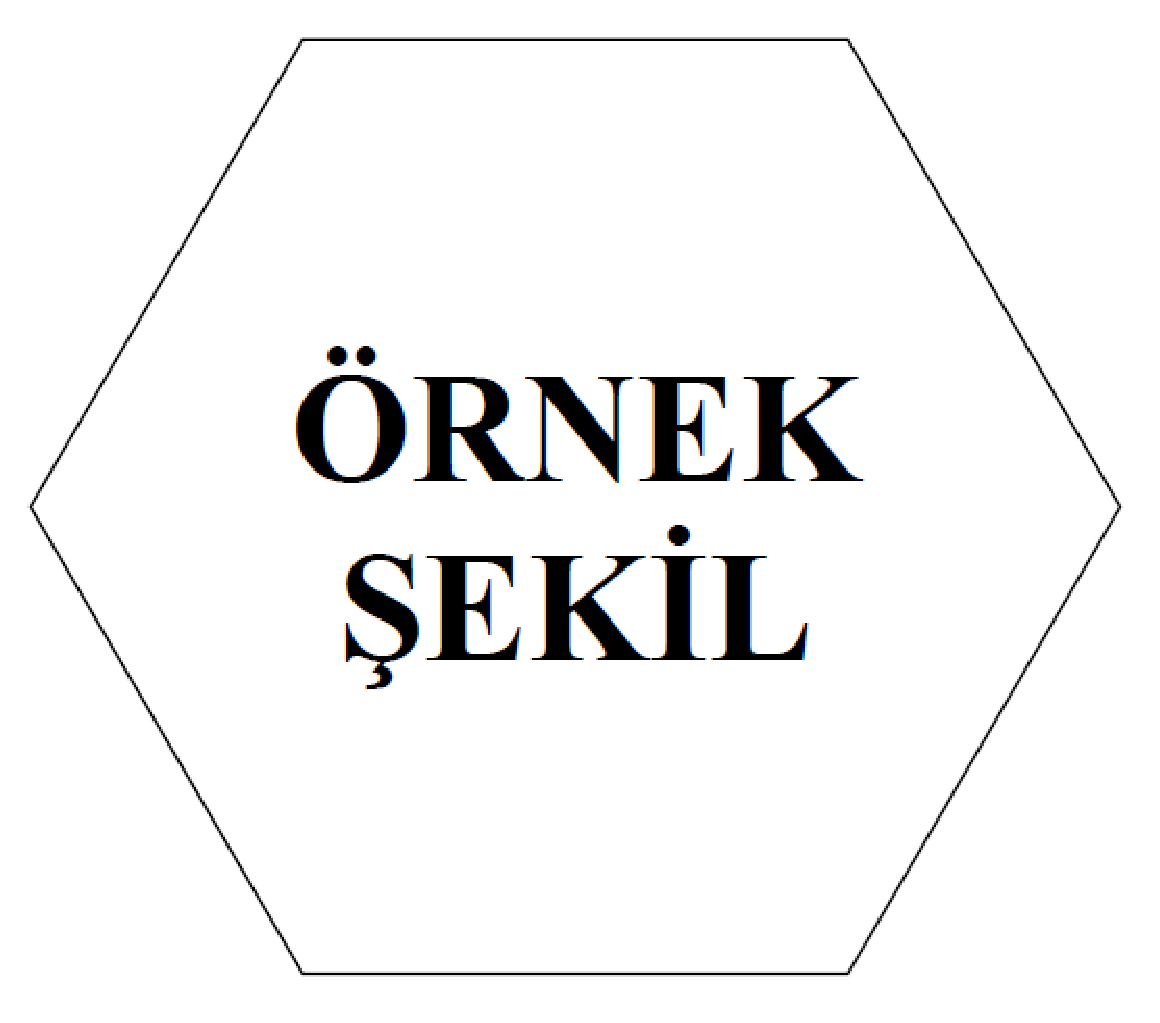
\includegraphics[width=230pt,keepaspectratio=true]{./fig/sekil6}
	% sekil6.eps: 0x0 pixel, 300dpi, 0.00x0.00 cm, bb=14 14 555 489
	\caption{For a multi-line figure captions, it is important that all the
		lines of the caption are aligned.}
	\label{fig:4-1}
\end{figure}

Lorem ipsum dolor sit amet, consectetur adipiscing elit. Sed ac augue vel dui 
adipiscing placerat et nec metus. Donec bibendum sodales mollis. Cras in lacus 
justo, at vestibulum quam. Sed semper, est sit amet consectetur ornare, leo est 
lacinia velit, adipiscing elementum lectus felis at sem.

\begin{table*}
	{\setlength{\tabcolsep}{14pt}
		\caption{Example table.}
		\begin{center}
			\vspace{-6mm}
			\begin{tabular}{cccc}
				\hline\hline
				Column A & Column B & Column C & Column D \\
				\hline
				Row A & Row A & Row A & Row A \\
				Row B & Row B & Row B & Row B \\
				Row C & Row C & Row C & Row C \\
				\hline
			\end{tabular}
			\vspace{-6mm}
		\end{center}
		\label{tableforCh4-1}}
\end{table*}

Lorem ipsum dolor sit amet, consectetur adipiscing elit. Sed ac augue vel dui 
adipiscing placerat et nec metus. Donec bibendum sodales mollis. Cras in lacus 
justo, at vestibulum quam. Sed semper, est sit amet consectetur ornare, leo est 
lacinia velit, adipiscing elementum lectus felis at sem. Aenean hendrerit erat eu 
lacus malesuada at sodales arcu egestas. Maecenas euismod urna ut sem luctus et 
congue metus vulputate. Ut pellentesque, neque eget fringilla elementum, ligula 
massa aliquet lorem, et varius nisi lacus vel diam. Etiam vitae metus sed orci 
rutrum fringilla. Phasellus sed velit quam. Mauris vestibulum, mauris a cursus 
adipiscing, nulla est hendrerit justo, ut fringilla eros velit ut mauris.
%%%%%%%%%%%%%%%%%%%%%%%%%%%%%%%%%%%%%%%%%%%%%%%%%%%%%%%%%%%%%%%%%
\chapter{(IF NECESSARY) CHAPTER 5}\label{ch:ifnecch5}
%%%%%%%%%%%%%%%%%%%%%%%%%%%%%%%%%%%%%%%%%%%%%%%%%%%%%%%%%%%%%%%%%

Lorem ipsum dolor sit amet, consectetur adipiscing elit. Sed ac augue vel dui 
adipiscing placerat et nec metus. Donec bibendum sodales mollis. Cras in lacus 
justo, at vestibulum quam. Sed semper, est sit amet consectetur ornare, leo est 
lacinia velit, adipiscing elementum lectus felis at sem. Aenean hendrerit erat eu 
lacus malesuada at sodales arcu egestas. Maecenas euismod urna ut sem luctus et 
congue metus vulputate. Ut pellentesque, neque eget fringilla elementum, ligula 
massa aliquet lorem, et varius nisi lacus vel diam. Etiam vitae metus sed orci 
rutrum fringilla. Phasellus sed velit quam. Mauris vestibulum, mauris a cursus 
adipiscing, nulla est hendrerit justo, ut fringilla eros velit ut mauris.

\section{Practical Application of This Study}

Lorem ipsum dolor sit amet, consectetur adipiscing elit. Sed ac augue vel dui 
adipiscing placerat et nec metus. Donec bibendum sodales mollis. Cras in lacus 
justo, at vestibulum quam. Sed semper, est sit amet consectetur ornare, leo est 
lacinia velit, adipiscing elementum lectus felis at sem. Aenean hendrerit erat eu 
lacus malesuada at sodales arcu egestas. Maecenas euismod urna ut sem luctus et 
congue metus vulputate. Ut pellentesque, neque eget fringilla elementum, ligula 
massa aliquet lorem, et varius nisi lacus vel diam. Etiam vitae metus sed orci 
rutrum fringilla. Phasellus sed velit quam. Mauris vestibulum, mauris a cursus 
adipiscing, nulla est hendrerit justo, ut fringilla eros velit ut mauris.

\section{Second Level Title: First Letters Capital}

Lorem ipsum dolor sit amet, consectetur adipiscing elit. Sed ac augue vel dui 
adipiscing placerat et nec metus. Donec bibendum sodales mollis. Cras in lacus 
justo, at vestibulum quam. Sed semper, est sit amet consectetur ornare, leo est 
lacinia velit, adipiscing elementum lectus felis at sem. 

\subsection{Third level title: Only first letter capital}

Lorem ipsum dolor sit amet, consectetur adipiscing elit. Sed ac augue vel dui 
adipiscing placerat et nec metus. Donec bibendum sodales mollis. Cras in lacus 
justo, at vestibulum quam. Sed semper, est sit amet consectetur ornare, leo est 
lacinia velit, adipiscing elementum lectus felis at sem.

\subsubsection{Fourth level title: Only first letter capital}

Lorem ipsum dolor sit amet, consectetur adipiscing elit. Sed ac augue vel dui 
adipiscing placerat et nec metus. Donec bibendum sodales mollis. Cras in lacus 
justo, at vestibulum quam. Sed semper, est sit amet consectetur ornare, leo est 
lacinia velit, adipiscing elementum lectus felis at sem.

{\bf Fifth level title: No numbering after fourth level titles}

Lorem ipsum dolor sit amet, consectetur adipiscing elit. Sed ac augue vel dui 
adipiscing placerat et nec metus. Donec bibendum sodales mollis. Cras in lacus 
justo, at vestibulum quam. Sed semper, est sit amet consectetur ornare, leo est 
lacinia velit, adipiscing elementum lectus felis at sem.

\begin{figure}
	\centering
	
\includegraphics[width=230pt,keepaspectratio=true]{./fig/sekil5}
	% sekil5.eps: 0x0 pixel, 300dpi, 0.00x0.00 cm, bb=14 14 1193 701
	\caption{For a multi-line figure captions, it is important that all the
		lines of the caption are aligned.}
	
	\label{fig:5-1}
\end{figure}

Lorem ipsum dolor sit amet, consectetur adipiscing elit. Sed ac augue vel dui 
adipiscing placerat et nec metus. Donec bibendum sodales mollis. Cras in lacus 
justo, at vestibulum quam. Sed semper, est sit amet consectetur ornare, leo est 
lacinia velit, adipiscing elementum lectus felis at sem.

\begin{table*}
	{\setlength{\tabcolsep}{14pt}
		\caption{Example table in chapter 5.}
		\begin{center}
			\vspace{-6mm}
			\begin{tabular}{cccc}
				\hline\hline
				Column A & Column B & Column C & Column D \\
				\hline
				Row A & Row A & Row A & Row A \\
				Row B & Row B & Row B & Row B \\
				Row C & Row C & Row C & Row C \\
				\hline
			\end{tabular}
			\vspace{-6mm}
		\end{center}
		\label{tableforCh5-1}}
\end{table*}

Lorem ipsum dolor sit amet, consectetur adipiscing elit. Sed ac augue vel dui 
adipiscing placerat et nec metus. Donec bibendum sodales mollis. Cras in lacus 
justo, at vestibulum quam. Sed semper, est sit amet consectetur ornare, leo est 
lacinia velit, adipiscing elementum lectus felis at sem. Aenean hendrerit erat eu 
lacus malesuada at sodales arcu egestas. Maecenas euismod urna ut sem luctus et 
congue metus vulputate. Ut pellentesque, neque eget fringilla elementum, ligula 
massa aliquet lorem, et varius nisi lacus vel diam. Etiam vitae metus sed orci 
rutrum fringilla. Phasellus sed velit quam. Mauris vestibulum, mauris a cursus 
adipiscing, nulla est hendrerit justo, ut fringilla eros velit ut mauris.
%%%%%%%%%%%%%%%%%%%%%%%%%%%%%%%%%%%%%%%%%%%%%%%%%%%%%%%%%%%%%%%%%
\chapter{EQUIPMENT, SOFTWARE AND SERVICE ACQUISITION (IF ANY OF THOSE ARE NOT CURRENTLY AVAILABLE, THE MEANS OF ACQUISITION)}\label{Ch6}
%%%%%%%%%%%%%%%%%%%%%%%%%%%%%%%%%%%%%%%%%%%%%%%%%%%%%%%%%%%%%%%%%

Expected total cost and budget of the study must be computed, and the economical feasibility of the study must be analyzed.

\section{Practical Application of This Study}

Lorem ipsum dolor sit amet, consetetur sadipscing elitr, sed diam nonumy eirmod tempor invidunt ut labore et dolore magna aliquyam erat, sed diam voluptua. At vero eos et accusam et justo duo dolores et ea rebum. Stet clita kasd gub rgren, no sea takimata sanctus est Lorem ipsum dolor sit amet, consetetur sadipscing elitr, sed diam nonumy eirmod tempor invidunt ut lab ore sit et dolore magna.

\section{Second Level Title: First Letters Capital}

Lorem ipsum dolor sit amet, consetetur sadipscing elitr, sed diam nonumy eirmod tempor invidunt ut labore et dolore magna aliquyam erat, sed diam voluptua. At vero eos et accusam et justo duo dolores et ea rebum. Stet clita kasd gub rgren, no sea.

\subsection{Third level title: Only first letter capital}

Lorem ipsum dolor sit amet, consetetur sadipscing elitr, sed diam nonumy eirmod tempor invidunt ut labore et dolore magna aliquyam erat, sed diam voluptua. At vero eos et accusam et justo duo dolores et ea rebum. Stet clita kasd gub rgren, no sea.

\subsubsection{Fourth level title: Only first letter capital}

Stet clita kasd gub rgren, no sea takimata sanctus est Lorem ipsum dolor sit amet, consetetur sadipscing elitr, sed diam nonumy eirmod tempor invidunt ut lab ore sit et dolore magna.

This indicates that the ANN is accurate at base flow and flow height values lower then 3 m. 

\begin{table*}[!htbp]
	{\setlength{\tabcolsep}{14pt}
		\caption{Example table in chapter 6.}
		\begin{center}
			\vspace{-6mm}
			\begin{tabular}{cccc}
				\hline \\[-2.45ex] \hline \\[-2.1ex]
				Column A & Column B & Column C & Column D \\
				\hline \\[-1.8ex]
				Row A & Row A & Row A & Row A \\
				Row B & Row B & Row B & Row B \\
				Row C & Row C & Row C & Row C \\
				[-0ex] \hline
			\end{tabular}
			\vspace{-6mm}
		\end{center}
		\label{Table6.1}}
\end{table*}

Stet clita kasd gub rgren, no sea takimata sanctus est Lorem ipsum dolor sit amet, consetetur sadipscing elitr, sed diam nonumy eirmod tempor invidunt ut lab ore sit et dolore magna. Stet clita kasd gub rgren, no sea takimata sanctus est Lorem ipsum dolor sit amet, consetetur sadipscing elitr, sed diam nonumy eirmod tempor invidunt ut lab ore sit et dolore magna. Stet clita kasd gub rgren, no sea takimata sanctus est Lorem ipsum dolor sit amet, consetetur sadipscing elitr, sed diam nonumy eirmod tempor invidunt ut lab ore sit et dolore magna. 

Stet clita kasd gub rgren, no sea takimata sanctus est Lorem ipsum dolor sit amet, consetetur sadipscing elitr, sed diam nonumy eirmod tempor invidunt ut lab ore sit et dolore magna. 

%{\bf Fifth level title: No numbering after fourth level titles}
\subsubsubsection{Fifth level title: No numbering after fourth level titles}

Lorem ipsum dolor sit amet, consectetur adipiscing elit. Sed ac augue vel dui adipiscing placerat et nec metus. Donec bibendum sodales mollis. Cras in lacus justo, at vestibulum quam. Sed semper, est sit amet consectetur ornare, leo est lacinia velit, adipiscing elementum lectus felis at sem.

\begin{figure}
	\centering
	
\includegraphics[width=230pt,keepaspectratio=true]{./fig/sekil7}
	% sekil7.eps: 0x0 pixel, 300dpi, 0.00x0.00 cm, bb=14 14 455 369
	\caption{Example table in chapter 6.}
	\label{Figure6.1}
\end{figure}

Lorem ipsum dolor sit amet, consectetur adipiscing elit. Sed ac augue vel dui adipiscing placerat et nec metus. Donec bibendum sodales mollis. Cras in lacus justo, at vestibulum quam. Sed semper, est sit amet consectetur ornare, leo est lacinia velit, adipiscing elementum lectus felis at sem.

Stet clita kasd gub rgren, no sea takimata sanctus est Lorem ipsum dolor sit amet, consetetur sadipscing elitr, sed diam nonumy eirmod tempor invidunt ut lab ore sit et dolore magna. Stet clita kasd gub rgren, no sea takimata sanctus est Lorem ipsum dolor sit amet, consetetur sadipscing elitr, sed diam nonumy eirmod tempor invidunt ut lab ore sit et dolore magna. Stet clita kasd gub rgren, no sea takimata sanctus est Lorem ipsum dolor sit amet, consetetur sadipscing elitr, sed diam nonumy eirmod tempor invidunt ut lab ore sit et dolore magna. 

Stet clita kasd gub rgren, no sea takimata sanctus est Lorem ipsum dolor sit amet, consetetur sadipscing elitr, sed diam nonumy eirmod tempor invidunt ut lab ore sit et dolore magna. 


% ----------------------------------------------------------------- %
% Form thesis_bib.bib to contain your references in bibtex format   %
% use \cite command for citing your references.                     %
% ----------------------------------------------------------------- %

\bibliographystyle{thesis_itubib}      % Designed .bst file 
\bibliography{thesis_bib}			   % .bib file

% ----------------------------------------------------------------- %
% Appendix files. appendices_cover is the appendix title page.      %
% ----------------------------------------------------------------- %

\eklerkapak{}
\vglue20pt
\singlespacing
\textbf{APPENDIX A.1 :} Maps\\
\textbf{APPENDIX A.2 :} Other Maps\\
\newpage

% ----------------------------------------------------------------- %
% \eklerbolum{x} forms and appendix of x chapters. 				    %
% ----------------------------------------------------------------- %

\eklerbolum{0}
\vglue20pt
\chapter{APPENDIX A.1}

\begin{table*}[!ht]
	{\setlength{\tabcolsep}{14pt}
		\caption{Example table in appendix.}
		\begin{center}
			\vspace{-6mm}
			\begin{tabular}{cccc}
				\hline\hline
				Column A & Column B & Column C & Column D \\
				\hline
				Row A & Row A & Row A & Row A \\
				Row B & Row B & Row B & Row B \\
				Row C & Row C & Row C & Row C \\
				\hline
			\end{tabular}
			\vspace{-6mm}
		\end{center}
		\label{tableappendix}}
\end{table*}

\section*{APPENDIX A.2}

Lorem ipsum dolor sit amet, consectetur adipiscing elit. Sed ac augue vel dui 
adipiscing placerat et nec metus. Donec bibendum sodales mollis. Cras in lacus 
justo, at vestibulum quam. Sed semper, est sit amet consectetur ornare, leo est 
lacinia velit, adipiscing elementum lectus felis at sem.

\newpage









% ----------------------------------------------------------------- %
% The summary page                                                  %
% ----------------------------------------------------------------- %

\ozgecmis{\vspace*{10mm}
\setlength{\TPHorizModule}{10pt}
\setlength{\TPVertModule}{10pt}
\begin{textblock}{1}(43.25,15.75) % Photo is adusted flush to the right margin - SBÖ
	\begin{figure}[p]
		
\includegraphics[scale=0.35,keepaspectratio=true]{./fig/photo}
		% photo.eps: 0x0 pixel, 300dpi, 0.00x0.00 cm, bb=14 14 279 359
	\end{figure}	
\end{textblock}
\vspace*{30mm}
\textbf{Name Surname\makebox[2.155cm]{\hfill \textbf{:}}}\hspace{0.225em} \\ % Adjust the colomn alignment - SBÖ

\vspace{-3mm}
\textbf{Place and Date of Birth\makebox[0.735cm]{\hfill \textbf{:}}}\hspace{0.225em} \\ % Adjust the colomn alignment - SBÖ

\vspace{-3mm}
\textbf{E-Mail\makebox[3.685cm]{\hfill \textbf{:}}}\hspace{0.225em} \\ % Adjust the colomn alignment - SBÖ

\vspace{5mm}

\renewcommand\labelitemi{\normalsize$\bullet$} 			% Adjust the size of the bullets - SBÖ

\textbf{EDUCATION\makebox[2.41cm]{\hfill \textbf{:}}}  	% Adjust the colomn alignment - SBÖ
\vspace{-3mm}

\begin{itemize}[leftmargin=5.15cm,itemsep=-0.25em,labelsep=2mm] % Adjust margin to flush left, item sep., label sep. - SBÖ
	\item [$\bullet$ \hspace{1em}\textbf{B.Sc.} \hspace{6.85em} \textbf{:}] Graduation year, Istanbul Technical University, Faculty of Electrical and Electronics, Department of Electrical Engineering
	\item [$\bullet$ \hspace{1em}\textbf{M.Sc. \textcolor{red}{(If exists)}} \hspace{2.4em} \textbf{:}] Graduation year, Istanbul Technical University, Faculty of Electrical and Electronics, Department of Electrical Engineering
\end{itemize}

\textbf{PROFESSIONAL EXPERIENCE AND REWARDS:}   
\vspace{-3mm}
\begin{itemize}[leftmargin=0.7cm,itemsep=-0.25em,labelsep=5mm] % Adjust margin to flush left, item sep., label sep. - SBÖ
	%\setlength{\itemindent}{-0.25em}
	\item 1950-1956 Istanbul Technical University at the Central Laboratory of Theoretical Physics.
	\item 1953 Nobel Prize for Physics
	\item 1956 Completed Doctorate at Istanbul Technical University
\end{itemize}

\textbf{PUBLICATIONS, PRESENTATIONS AND PATENTS ON THE THESIS:} 
\vspace{-3mm}
\begin{itemize}[leftmargin=0.7cm,itemsep=0.5em,labelsep=5mm] % Adjust margin to flush left, item sep., label seperation - SBÖ
	%\setlength{\itemindent}{-0.25em}
	\item \textbf{Ganapuram S., Hamidov A., Demirel, M. C., Bozkurt E., Kındap U., Newton A.} % Bold authors font - SBÖ
	2007. Erasmus Mundus Scholar's Perspective On Water And Coastal
	Management Education In Europe. 
	\textit{International Congress - River Basin Management}, 
	March 22--24, 2007 Antalya, Turkey. \textcolor{red}{(Presentation Instance)}
	
	\item \textbf{Satoğlu, Ş.I., Durmuşoğlu, M. B., Ertay, T. A.} 2010. A Mathematical Model  % Bold authors font - SBÖ
	And A Heuristic Approach For Design Of The Hybrid Manufacturing Systems 
	To Facilitate One-Piece Flow, 
	\textit{International Journal of Production Research,}
	48(17), 5195--5220. \textcolor{red}{(Article Instance)}
	
	\item  \textbf{Chen, Z.} 2013. Intelligent Digital Teaching And Learning All-In-One Machine, % Bold authors font - SBÖ
	Has Projection Mechanism Whose Front End Is Connected With Supporting
	Arm, And Base Shell Provided With Panoramic Camera That Is Connected With
	Projector. Patent numarası: CN203102627-U. \textcolor{red}{(Patent Instance)}
\end{itemize}

%\newpage

\textbf{OTHER PUBLICATIONS, PRESENTATIONS AND PATENTS:} 
\vspace{-3mm}
% ---------------------------------------------------------------- %
% Fotografli ve yayin listeli (yayini varsa) ozgecmis onerilir.    %
% Fotograf ve adres sart degildir.				                   %
% ---------------------------------------------------------------- %

%======================================== SIRT OF THE THESIS ========================================= - SBÖ
\newpage % Last page is assigned for the SIRT of the Thesis 
\thispagestyle{empty} % Remove the bottom page number
% Definitions in sırt of the thesis
\def\sirtyili{2020} % Year of the graduation
\def\studentname{F. M. SURNAME} % F. and M. initials SURNAME
\def\thesisthickness{25mm} % Enter the expected thickness of the thesis after the hardcover 

\hspace*{75mm}
\begin{tikzpicture}[remember picture,overlay]
{\rotatebox[origin=c,x=23.35mm,y=-247.75mm]{90}{\draw [line width=0.01mm, black, dashed] (0mm,0mm) rectangle node{\normalsize \studentname} (65mm,\thesisthickness);}}

{\rotatebox[origin=c,x=23.35mm,y=-247.75mm]{90}{\draw [line width=0.01mm, black ,dashed, text width=190mm, align=center] (67mm,0mm) rectangle node{\normalsize \Baslikspacing \Baslikbir~\Baslikiki~\Baslikuc} (193mm+65mm+2mm,\thesisthickness);}}

{\rotatebox[origin=c,x=23.35mm,y=-247.75mm]{90}{\draw [line width=0.01mm, black ,dashed] (193mm+65mm+4mm,0mm) rectangle node{\normalsize \sirtyili} (296.5mm,\thesisthickness);}}

{\rotatebox[origin=c,x=23.35mm,y=-247.75mm]{90}{\draw[black,line width=1mm] (64.5mm,0mm) -- (64.5mm,\thesisthickness);
\draw[black,line width=1mm] (67.3mm,0mm) -- (67.3mm,\thesisthickness);
}}

{\rotatebox[origin=c,x=23.35mm,y=-247.75mm]{90}{\draw[black,line width=1mm] (193mm+64.5mm+2mm,0mm) -- (193mm+64.5mm+2mm,\thesisthickness);
\draw[black,line width=1mm] (193mm+64.5mm+5mm,0mm) -- (193mm+64.5mm+5mm,\thesisthickness);
}}
% Four dashed lines added between double thick lines vertically
\draw [line width=0.01mm, black, dashed] (0mm,-205mm) -- (0mm,-208mm);
\draw [line width=0.01mm, black, dashed] (-\thesisthickness,-205mm) -- (-\thesisthickness,-208mm);
\draw [line width=0.01mm, black, dashed] (0mm,-3.25mm) -- (0mm,-13mm);
\draw [line width=0.01mm, black, dashed] (-\thesisthickness,-1mm) -- (-\thesisthickness,-13mm);
\end{tikzpicture}} % Edge (Sırt) of the thesis at the very end.
\end{document}                      

% ----------------------------------------------------------------- %
% About this template: iletisim@be.itu.edu.tr                       %
% Updated by	:													%
% E. Baris Ondes: ondes@itu.edu.tr 	 OR ondesalt@pm.me				% 
% Tamer Sener	: senerta@itu.edu.tr OR tamsener@gmail.com			%
% Berkan Kacmaz	: kacmazb@itu.edu.tr OR kacmazberkan0@gmail.com		%
% S. Baris Ozturk : ozturksb@itu.edu.tr OR salihbaris@gmail.com		%
% ----------------------------------------------------------------- %